%% History:
% Pavel Tvrdik (26.12.2004)
%  + initial version for PhD Report
%
% Daniel Sykora (27.01.2005)
%
% Michal Valenta (3.12.2008)
% rada zmen ve formatovani (diky M. Duškovi, J. Holubovi a J. Žďárkovi)
% sjednoceni zdrojoveho kodu pro anglickou, ceskou, bakalarskou a diplomovou praci

% One-page layout: (proof-)reading on display
%%%% \documentclass[11pt,oneside,a4paper]{book}
% Two-page layout: final printing
\documentclass[11pt,twoside,a4paper]{book}   
%=-=-=-=-=-=-=-=-=-=-=-=--=%
% The user of this template may find useful to have an alternative to these 
% officially suggested packages:
\usepackage[czech, english, slovak]{babel}
\usepackage[T1]{fontenc} % pouzije EC fonty 
\usepackage{longtable}
% pripadne pisete-li cesky, pak lze zkusit take:
% \usepackage[OT1]{fontenc} 
\usepackage[utf8]{inputenc}
%=-=-=-=-=-=-=-=-=-=-=-=--=%
% In case of problems with PDF fonts, one may try to uncomment this line:
%\usepackage{lmodern}
%=-=-=-=-=-=-=-=-=-=-=-=--=%
%=-=-=-=-=-=-=-=-=-=-=-=--=%
% Depending on your particular TeX distribution and version of conversion tools 
% (dvips/dvipdf/ps2pdf), some (advanced | desperate) users may prefer to use 
% different settings.
% Please uncomment the following style and use your CSLaTeX (cslatex/pdfcslatex) 
% to process your work. Note however, this file is in UTF-8 and a conversion to 
% your native encoding may be required. Some settings below depend on babel 
% macros and should also be modified. See \selectlanguage \iflanguage.
%\usepackage{czech}  %%%%%\usepackage[T1]{czech} %%%%[IL2] [T1] [OT1]
%=-=-=-=-=-=-=-=-=-=-=-=--=%

%%%%%%%%%%%%%%%%%%%%%%%%%%%%%%%%%%%%%%%
% Styles required in your work follow %
%%%%%%%%%%%%%%%%%%%%%%%%%%%%%%%%%%%%%%%
\usepackage{graphicx}
%\usepackage{indentfirst} %1. odstavec jako v cestine.

\usepackage{k336_thesis_macros} % specialni makra pro formatovani DP a BP
 % muzete si vytvorit i sva vlastni v souboru k336_thesis_macros.sty
 % najdete  radu jednoduchych definic, ktere zde ani nejsou pouzity
 % napriklad: 
 % \newcommand{\bfig}{\begin{figure}\begin{center}}
 % \newcommand{\efig}{\end{center}\end{figure}}
 % umoznuje pouzit prikaz \bfig namisto \begin{figure}\begin{center} atd.


%%%%%%%%%%%%%%%%%%%%%%%%%%%%%%%%%%%%%
% Zvolte jednu z moznosti 
% Choose one of the following options
%%%%%%%%%%%%%%%%%%%%%%%%%%%%%%%%%%%%%
\newcommand\TypeOfWork{Diplomová práca} \typeout{Diplomova prace}
% \newcommand\TypeOfWork{Master's Thesis}   \typeout{Master's Thesis} 
% \newcommand\TypeOfWork{Bakalářská práce}  \typeout{Bakalarska prace}
% \newcommand\TypeOfWork{Bachelor's Project}  \typeout{Bachelor's Project}


%%%%%%%%%%%%%%%%%%%%%%%%%%%%%%%%%%%%%
% Zvolte jednu z moznosti 
% Choose one of the following options
%%%%%%%%%%%%%%%%%%%%%%%%%%%%%%%%%%%%%
% nabidky jsou z: http://www.fel.cvut.cz/cz/education/bk/prehled.html

%\newcommand\StudProgram{Elektrotechnika a informatika, dobíhající, Bakalářský}
%\newcommand\StudProgram{Elektrotechnika a informatika, dobíhající, Magisterský}
% \newcommand\StudProgram{Elektrotechnika a informatika, strukturovaný, Bakalářský}
 \newcommand\StudProgram{Otvorená informatika, Magisterský}
% \newcommand\StudProgram{Softwarové technologie a management, Bakalářský}
% English study:
% \newcommand\StudProgram{Electrical Engineering and Information Technology}  % bachelor programe
% \newcommand\StudProgram{Electrical Engineering and Information Technology}  %master program


%%%%%%%%%%%%%%%%%%%%%%%%%%%%%%%%%%%%%
% Zvolte jednu z moznosti 
% Choose one of the following options
%%%%%%%%%%%%%%%%%%%%%%%%%%%%%%%%%%%%%
% nabidky jsou z: http://www.fel.cvut.cz/cz/education/bk/prehled.html

%\newcommand\StudBranch{Výpočetní technika}   % pro program EaI bak. (dobihajici i strukt.)
\newcommand\StudBranch{Softwarové inžinierstvo}   % pro prgoram EaI mag. (dobihajici i strukt.)
%\newcommand\StudBranch{Softwarové inženýrství}            %pro STM
%\newcommand\StudBranch{Web a multimedia}                  % pro STM
%\newcommand\StudBranch{Computer Engineering}              % bachelor programe
%\newcommand\StudBranch{Computer Science and Engineering}  % master programe


%%%%%%%%%%%%%%%%%%%%%%%%%%%%%%%%%%%%%%%%%%%%
% Vyplnte nazev prace, autora a vedouciho
% Set up Work Title, Author and Supervisor
%%%%%%%%%%%%%%%%%%%%%%%%%%%%%%%%%%%%%%%%%%%%

\newcommand\WorkTitle{Veľkoobjemové úložisko emailov}
\newcommand\FirstandFamilyName{Bc. Patrik Lenárt}
\newcommand\Supervisor{Ing. Jan Šedivý, CSc.}


% Pouzijete-li pdflatex, tak je prijemne, kdyz bude mit vase prace
% funkcni odkazy i v pdf formatu
\usepackage[
pdftitle={\WorkTitle},
pdfauthor={\FirstandFamilyName},
bookmarks=true,
colorlinks=true,
breaklinks=true,
urlcolor=red,
citecolor=blue,
linkcolor=blue,
unicode=true,
]
{hyperref}



% Extension posted by Petr Dlouhy in order for better sources reference (\cite{} command) especially in Czech.
% April 2010
% See comment over \thebibliography command for details.

\usepackage[square, numbers]{natbib}             % sazba pouzite literatury


\usepackage{enumerate}
\usepackage{multirow}
\usepackage{booktabs}
\usepackage{capt-of} 


%\usepackage{url}
%\DeclareUrlCommand\url{\def\UrlLeft{<}\def\UrlRight{>}\urlstyle{tt}}  %rm/sf/tt
%\renewcommand{\emph}[1]{\textsl{#1}}    % melo by byt kurziva nebo sklonene,
\let\oldUrl\url
\renewcommand\url[1]{<\texttt{\oldUrl{#1}}>}




\begin{document}

%%%%%%%%%%%%%%%%%%%%%%%%%%%%%%%%%%%%%
% Zvolte jednu z moznosti 
% Choose one of the following options
%%%%%%%%%%%%%%%%%%%%%%%%%%%%%%%%%%%%%
\selectlanguage{slovak}
%\selectlanguage{english} 

% prikaz \typeout vypise vyse uvedena nastaveni v prikazovem okne
% pro pohodlne ladeni prace


\iflanguage{slovak}{
	 \typeout{************************************************}
	 \typeout{Zvoleny jazyk: cestina}
	 \typeout{Typ prace: \TypeOfWork}
	 \typeout{Studijni program: \StudProgram}
	 \typeout{Obor: \StudBranch}
	 \typeout{Jmeno: \FirstandFamilyName}
	 \typeout{Nazev prace: \WorkTitle}
	 \typeout{Vedouci prace: \Supervisor}
	 \typeout{***************************************************}
	 \newcommand\Department{Katedra počítačové grafiky a interakce}
	 \newcommand\Faculty{Fakulta elektrotechnická}
	 \newcommand\University{České vysoké učení technické v Praze}
	 \newcommand\labelSupervisor{Vedúci práce}
	 \newcommand\labelStudProgram{Študijný program}
	 \newcommand\labelStudBranch{Odbor}
}{
	 \typeout{************************************************}
	 \typeout{Language: english}
	 \typeout{Type of Work: \TypeOfWork}
	 \typeout{Study Program: \StudProgram}
	 \typeout{Study Branch: \StudBranch}
	 \typeout{Author: \FirstandFamilyName}
	 \typeout{Title: \WorkTitle}
	 \typeout{Supervisor: \Supervisor}
	 \typeout{***************************************************}
	 \newcommand\Department{Department of Computer Science and Engineering}
	 \newcommand\Faculty{Faculty of Electrical Engineering}
	 \newcommand\University{Czech Technical University in Prague}
	 \newcommand\labelSupervisor{Supervisor}
	 \newcommand\labelStudProgram{Study Programme} 
	 \newcommand\labelStudBranch{Field of Study}
}




%%%%%%%%%%%%%%%%%%%%%%%%%%    Poznamky ke kompletaci prace
% Nasledujici pasaz uzavrenou v {} ve sve praci samozrejme 
% zakomentujte nebo odstrante. 
% Ve vysledne svazane praci bude nahrazena skutecnym 
% oficialnim zadanim vasi prace.
{
\pagenumbering{roman} \cleardoublepage \thispagestyle{empty}
\chapter*{Na tomto místě bude oficiální zadání vaší práce}
\begin{itemize}
\item Toto zadání je podepsané děkanem a vedoucím katedry,
\item musíte si ho vyzvednout na studiijním oddělení Katedry počítačů na Karlově náměstí,
\item v jedné odevzdané práci bude originál tohoto zadání (originál zůstává po obhajobě na katedře),
\item ve druhé bude na stejném místě neověřená kopie tohoto dokumentu (tato se vám vrátí po obhajobě).
\end{itemize}
\newpage
}

%%%%%%%%%%%%%%%%%%%%%%%%%%    Titulni stranka / Title page 

\coverpagestarts

%%%%%%%%%%%%%%%%%%%%%%%%%%%    Podekovani / Acknowledgements 

\acknowledgements
\noindent
Rád by som poďakoval vedúcemu práce pánovi Ing. Janovi Šedivému, CSc. za konzultácie, cenné rady, pripomienky a návrhy, ktoré mi ochotne poskytol počas vypracovávania tejto práce. Tak isto sa chcem poďakovať svojim najbližším, bez ktorých podpory by táto práca nevznikla.



%%%%%%%%%%%%%%%%%%%%%%%%%%%   Prohlaseni / Declaration 

\declaration{V Prahe dňa 10.\,5.\,2011}
%\declaration{In Kořenovice nad Bečvárkou on May 15, 2008}


%%%%%%%%%%%%%%%%%%%%%%%%%%%%    Abstract 
 
\abstractpage

Translation of Czech abstract into English.

% Prace v cestine musi krome abstraktu v anglictine obsahovat i
% abstrakt v cestine.
\vglue60mm

\noindent{\Huge \textbf{Abstrakt}}
\vskip 2.75\baselineskip

\noindent

Cieľom tejto práce je návrh riešenia pre archiváciu elektronickej pošty s využitím distribuovaných databázových systémov, ktoré sa označujú pod spoločným názvom NoSQL. Analýzovali sme požiadavky na veľkoobjemový a vysokodostupný archív emailových správ, ktorý bude z dôvodu úspory diskového priestoru využívať deduplikáciu príloh. V práci popisujeme základné koncepty, ktoré sa využívajú pri tvorbe distribuovaných databázových systémov. Stanovili sme základné kritéria na porovnanie NoSQL systémov, z ktorých sme následne vybrali dvoch kandidátov, spĺňajúcich požiadavky systému. Popísali sme funkcionalitu systémov Cassandra a HBase, ktoré sme podrobili výkonnostným testom. Navrhli sme model a implemetovali prototyp aplikácie využivajúci systém Cassandra. Po naplnení systému približne miliónom emailových správ, z reálneho prostredia, sme vďaka použitiu deduplikácie dosiahli cca 65\% úsporu diskového priestoru.

%Navrhli sme model a pomocou systému Cassandra sme následne implemetovali prototyp aplikácie, u ktorého sme vďaka použitiu deduplikácie dosiahli 60\% úsporu diskového priestoru, pri naplnení systému približne miliónom emailových správ z reálneho prostredia.
%aktuálne problémy, ktoré vznikajú pri ukladaní a spracúvani neustále narastajúceho objemu dát pomocou relačných databázových systémov. Na ich riešenie 


%Cieľom tejto práce je návrh riešenia pre archiváciu elektronickej pošty s využitím distribuovaných databázových systémov, ktoré sa označujú pod spoločným názvom NoSQL. Analyzujeme požiadavky na veľkoobjemový a vysokodostupný archív emailových správ, ktorý bude z dôvodu úspory diskového priestoru využívať deduplikáciu. Skúmaním relačných databázových technológii sme identifikovali kritické body, na základe ktorých tieto systémy nespĺňaju naše požiadavky. Ako alternatívne riešenie volíme použitie NoSQL systémov, ktoré sa snažíme kategorizovať a následne z nich vybrať najhodnejších kandidátov pre požiadavky nášho systému. Zaoberáme sa architektúrou systémov Cassandra a HBase, ktoré podrobíme výkonnostným testom. Navrhli sme model a pomocou systému Cassandra sme následne implemetovali prototyp aplikácie. Po naplnení systému približne miliónom emailových správ, z reálneho prostredia, sme vďaka použitiu deduplikácie dosiahli 60\% úsporu diskového priestoru.


%%%%%%%%%%%%%%%%%%%%%%%%%%%%%%%%  Obsah / Table of Contents 

\tableofcontents


%%%%%%%%%%%%%%%%%%%%%%%%%%%%%%%  Seznam obrazku / List of Figures 

\listoffigures


%%%%%%%%%%%%%%%%%%%%%%%%%%%%%%%  Seznam tabulek / List of Tables

\listoftables


%**************************************************************

\mainbodystarts
% horizontalní mezera mezi dvema odstavci
%\parskip=5pt
%11.12.2008 parskip + tolerance
\normalfont
\parskip=0.2\baselineskip plus 0.2\baselineskip minus 0.1\baselineskip

% Odsazeni prvniho radku odstavce resi class book (neaplikuje se na prvni 
% odstavce kapitol, sekci, podsekci atd.) Viz usepackage{indentfirst}.
% Chcete-li selektivne zamezit odsazeni 1. radku nektereho odstavce,
% pouzijte prikaz \noindent.

%**************************************************************

% Pro snadnejsi praci s vetsimi texty je rozumne tyto rozdelit
% do samostatnych souboru nejlepe dle kapitol a tyto potom vkladat
% pomoci prikazu \include{jmeno_souboru.tex} nebo \include{jmeno_souboru}.
% Napr.:
% \include{1_uvod}
% \include{2_teorie}
% atd...

%*****************************************************************************
\chapter{Úvod}
%Úvod charakterizující kontext zadání, případně motivace.
S neustálym rozvojom informačných technológií súčasne narastá objem informácií, ktoré je potrebné spracúvať. Tento fakt podnietil vznik databázových systémov, ktoré slúžia na organizáciu, uchovávanie a spracovanie dát. V dnešnej dobe existuje veľké množstvo databázových systémov, ktoré sa navzájom líšia napríklad architektúrou, dátovým modelom alebo výrobcom.

Od začiatku sedemdesiatych rokov 20. storočia sú v tejto oblasti dominantou relačné databázové systémy (Relational Database Management Systems). Z dôvodu rapídneho rastu dát v digitálnom univerze \cite{Gantz_Mcarthur_Minton_2007} začínajú byť tieto systémy nepostačujúce. Medzi hlavné faktory pre výber relačného databázového systému doposiaľ patrili výrobca, cena a pod. Vznikajúce moderné webové aplikácie (napríklad sociálne siete) požadujú od týchto systémov vlastnosti ako vysoká dostupnosť, horizontálna rozšíriteľnosť a schopnosť pracovať s obrovským objemom dát (PB, petabajt\footnote{$ 1PB = 10^{15} B$}). Novo vznikajúce databázové systémy, spĺňajúce tieto požiadavky sa spoločne označujú pod názvom NoSQL (Not Only SQL). Pri ich výbere je dôležité porozumenie architektúry, dátového modelu a dát, s ktorými budú tieto systémy pracovať.

Táto práca si kladie za cieľ viacero úloh a je rozdelená do troch logických častí. V prvej časti popisujeme v kapitole 2, koncepty využívané pri tvorbe distribuovaných databázových systémov, ktoré zabezpečujú vysokú dostupnosť, spoľahlivosť a škálovateľnosť. Kapitola 3 definuje požiadavky na systém, schopný archivovať milióny emailových správ a tieto dáta ďalej spracúvať. Prehľad systémov NoSQL a kritéria pre ich porovnanie popisuje kapitola 4, ktorá v závere doporučuje výber dvoch vhodných kandidátov, systém Cassandra a HBAse. Architektonické princípy, z ktorých tieto systémy vychádzajú a ich vlastnosti sú popísané v kapitole 5 pre systém Cassandra a v kapitole 6 pre HBase.
%TODO: kapitola 8 + popis implementacie
V druhej časti práce v kapitole 7 sme vykonali výkonostné porovnanie týchto dvoch systémov zamerané na operáciu zápisu dát. Návrh modelu systému, výber vhodných nástrojov pre implementáciu prototypu aplikácie emailového úložiska a popisuje kapitola 8. 

Záverečná čast, ktorú tvorí kapitola 9 popisuje dosiahnuté výsledky a doporučuje systém pre riešenie danej úlohy.





%Výsledná struktura vaší práce a názvy a rozsahy jednotlivých kapitol se samozřejmě budou lišit podle typu práce a podle konkrétní povahy zpracovávaného tématu. Níže uvedená struktura práce odpovídá \textit{práci implementační}, viz \cite{infodp} respektive \cite{infobp}. 


\chapter{Databázové systémy}

V tejto časti stručne popíšeme históriu vzniku databázových systémov. Identifikujeme problémy spojené so škálovaním relačných databázových systémov a uvedieme možné spôsoby ich riešenia. Ďalej popíšeme základné koncepty využívané pri tvorbe distribuovaných databázových systémov a techniku MapReduce, ktorá slúži na paralelné spracovanie veľkého objemu dát (PB).

\section{História}

V polovici šesťdesiatych rokov 20. storočia bol spoločnosťou IBM vytvorený informačný systém IMS (Information Management System), využívajúci hierarchichký databázový model. IMS je po rokoch vývoja využívaný dodnes. Po krátkej dobe, v roku 1970, publikoval zamestnanec IBM, Dr. Edger F. Codd článok pod názvom „A Relational Model of Data for Large Shared Data Banks“ \cite{Codd:1970:RMD:362384.362685}, ktorým uviedol relačný databázový model. Prvým databázovým systémom implementujúcim tento model bol System R od IBM. Systém používal jazyk pod názvom SEQUEL, ktorý je predchodca dnešného SQL (Structured Query Language) slúžiaceho na manipuláciu a definíciu dát v relačných databázových systémoch. Tento koncept sa stal základom pre relačné databázové systémy, ktoré vďaka širokej škále vlastností (ako napríklad podpora transakcií a dotazovací jazyk SQL) patria v dnešnej  dobe medzi najpouživanejšie riešenia na trhu.

V minulosti boli objem dát, s ktorým tieto systémy pracovali menší a výkon hardvéru mnohonásobne nižší. Dnes napriek tomu, že výkon procesorov a veľkosť pamäťových zariadení rapídne stúpa, je najväčšou slabinou počítačových systémov rýchlosť prenosu dát medzi pevným diskom a operačnou pamäťou. Tento fakt je kritický pre novovznikajúce webové aplikácie ako napríklad sociálne siete alebo \emph{cloudové systémy}, ktoré majú neustále vyššie nároky na spracovávaný objem dát v reálnom čase a vyžadujú podporu škálovania, ktorá zabezpečuje vysokú dostupnosť a spoľahlivosť. Tieto požiadavky sa snažia efektívne riešiť novovznikajúce distribuované systémy pod spoločným názvom NoSQL, ktoré sú popísané v štvrtej kapitole tejto práce. %\ref{chapter:NoSQL}. 
%TODO ref na 4kap


%Novo vznikajúce webové aplikácie ako napríklad sociálne siete a zavádzanie \emph{cloud computingu} majú neustále vyššie nároky na spracovávaný objem dát, od systémov vyžadujú podporu škálovania, ktorá zabezpečuje vysokú dostupnosť a spoľahlivosť. Tieto nové požiadavky sa snažia efektívne riešiť distribuované systémy pod spoločným názvom NoSQL, ktoré sú popísané štvrtej kapitole tejto práce. 
\section{Distribuované databázové systémy}
Distribuovaný databázový systém je tvorený pomocou viacerých samostatne operujúcich databázových systémov, ktoré nazývame uzly a ich komunikácia sa vykonáva prostredníctvom počítačovej siete. Užívateľovi alebo aplikácii sa javia ako jeden celok \cite{hewitt2010cassandra}. Poďla konfigurácie jednotlivých uzlov v systéme ich ďalej delíme na:
\begin{itemize}
 \item distribuované databázove systémy typu \uv{master-slave}
 \item decentralizované distribuované databázové systémy
\end{itemize}

\subsection*{Systémy master-slave} 

Táto konfigurácia obsahuje uzol \emph{master}, ktorý plní jedinečnú úlohu a všetky uzly typu \emph{slave} sú na ňom závislé. V prípade jeho havárie je ohrozená funkčnosť celého systému, nazývame ho kritický bod výpadku (SPOF, single point of failure). Túto konfiguráciu uzlov používajú napríklad relačné databázové systémy.

\subsection*{Decentralizované systémy}

Pod názvom decentralizácia sa myslí, že každý uzol v distribuovanom databázovom systémy vykonáva tú istú úlohu a je kedykoľvek nahraditeľný. Táto konfigurácia neobsahuje SPOF.


\section{ACID}

Relačné databázové systémy poskytujú veľkú množinu operácií, ktoré je možné vykonávať nad dátami v nich uloženými. Transakcie \cite{gray1981transaction, haerder1983principles} sú zodpovedné za korektné vykonanie operácií v prípade, že spĺňajú množinu vlastností ACID. Význam jednotlivých vlastností akronymu ACID je následovný:

\begin{itemize}
  \item \emph{Atomicita} (Atomicity) - zaisťuje, že sa vykonajú všetky operácie reprezentujúce transakciu, čo spôsobí korektný prechod systému do nového stavu. V prípade zlyhania transakcie nemá daná operácia žiaden vplyv na výsledný stav systému a prechod do nového stavu sa nevykoná.
  \item \emph{Konzistencia} (Consistency) - každá transakcia po svojom úspešnom ukončení garantuje korektnosť svojho výsledku a zabezpečí, že systém prejde z jedného konzistentného stavu do druhého. Konzistentný stav zaručuje, že dáta v systéme odpovedajú požadovanej hodnote. Systém sa musí nachádzať v konzistentnom stave aj v prípade zlyhania transakcie.
  \item \emph{Izolácia} (Isolation) - operácie, ktoré prebiehajú počas vykonávania jednej transakcie nie sú viditeľné ostatným. Operácie tvoriace transakciu musia mať konzistentný prístup k dátam a to aj v prípade, že u inej transakcie dôjde k jej zlyhaniu.
  \item \emph{Trvácnosť} (Durability) - v prípade, že bola transakcia úspešne ukončená, systém musí garantovať trvácnosť jej výsledku aj v prípade svojho zlyhania.
\end{itemize}
%http://en.wikipedia.org/wiki/Concurrency_control#Concurrency_control_mechanisms
%http://en.wikipedia.org/wiki/Multiversion_concurrency_control
%http://en.wikipedia.org/wiki/Timestamp-based_concurrency_control
Implementácia vlastností ACID, ktoré zaručujú konzistenciu, zvyčajne využíva u relačných databázových systémov metódu zamykania. Transakcia uzamkne dáta pred ich spracovaním a spôsobí ich nedostupnosť až do jej úspešného ukončenia, poprípade zlyhania. Tranzakcie sú vykonávané sekvenčne. Pre databázový systém, od ktoréhu požadujeme vysokú dostupnosť tento model nie je vyhovujúci. Zámky spôsobujú stavy, kedy ostatné transakcie musia čakať na ich uvoľnenie. Náhradou je mechanizmus s názvom \uv{riadenie súbežného spracovania s viacerými verziami} (MVCC, Multiversion concurrency control), ktorý umožnuje paralelné vykonávanie operácií nad dátami, jeho popis obsahuje práca od P. Bernsteina a N. Goodmana \cite{bernstein1981concurrency}. Tento mechanizmus je zárovenň využívaný systémami NoSQL.


%http://en.wikipedia.org/wiki/2-phase_commit
%http://en.wikipedia.org/wiki/Two-phase_locking
% a operácií spojenia (join) 
Tranzakcie splňujúce vlastnosti ACID využívajú v distribuovaných databázových systémoch dvojfázový potvrdzovací protokol (Two-phase commit protocol \cite{bernstein1987concurrency}). Systém využívajúci tento protokol, zaručuje konzistentnosť a je schopný odolávať sieťovým prerušeniam (network partitioning) alebo poruchám v systéme. Vlastnosti ACID nekladú žiadnu záruku na dostupnosť systému, naopak nedostupnosť je uprednostnená v prípade operácie, ktorá by mohla spôsobiť nekonzistenciu dát. Takéto systémy sú vhodné pre aplikácie, v ktorých sa vykonávajú platobné operácie a pod. Existuje množstvo aplikácií, u ktorých sa uprednosňuje dostupnosť dát pred ich konzistenciou. Pri tvorbe distribuovaných databázových systémov je preto potrebné upustiť z niektorých ACID vlastností. Riešenie poskytuje model pod názvom BASE \ref{section:base}.

%ACID makes no guarantees regarding availability; indeed, it is preferable for an ACID service to be unavailable than to function in a way that relaxes the ACID constraints. ACID semantics are well suited for Internet commerce transactions, billing users, or maintaining user profile information for personalized services

\section{Škálovanie databázového systému} %scalepub04.pdf
Obecná definícia pojmu \emph{škálovateľnosť} \cite{bondi2000characteristics} je náročná  bez vymedzenia kontextu, ku ktorému sa vzťahuje. V tejto kapitole budeme pojem škálovateľnosť chápať v kontexte webových aplikácií, ktorých dynamický vývoj kladie na databázové systémy viacero požiadaviek. Definujme škálovatelnosť databázového systému ako vlastnosť, vďaka ktorej je systém schopný spracúvať požiadavky webovej aplikácie v definovanom časovom intervale. Medzi hlavné z týchto požiadavkov patrí vysoká dostupnosť, spoľahlivosť a odolnosť systému voči chybám. Typicky sa táto vlasnosť realizuje pridaním nových uzlov do aktuálneho systému s využitím replikácie. Aplikácia týchto mechanizmov má za následok využitie distribuovaného databázového systému. Škálovateľnosť delíme na vertikálnu, horizontálnu a systému dodáva ďalšie z nasledujúcich vlastnosti \cite{hewitt2010cassandra}:
\begin{itemize}
 \item umožňuje zväčšiť veľkosť celkovej kapacity databáze a táto zmena by mala byť transparentná z pohľadu aplikácie na dáta
  \item zvyšuje celkové množstvo operácií, pre čítanie a zápis dát, ktoré je systém schopný vykonať v danú časovú jednotku
  \item v určitých prípadoch môže zaručiť, že systém neobsahuje kritický bod výpadku
  \item zvyšuje celkovú dostupnosť systému
\end{itemize}

Vertikálna škálovateľnosť je metóda, ktorá sa aplikuje pomocou zvýšovania výkonnosti hardvéru, do systému sa pridáva operačná pamäť, rychlejšie viacjádrové procesory, zvyšuje sa kapacita diskov. Jednou z nevýhod tohoto riešenia je jeho vysoká cena a možná nedostupnosť systému v prípade jeho zlyhania.
Proces vertikálneho škálovania sa hlavne aplikuje v prípade použitia relačných databázových systémov  a obsahuje následujúce kroky:
\begin{itemize}
 \item zámena hardvéru za výkonnejší
 \item úprava súborového systému (napr. zrušenie žurnálu a uchovávania informácie o poslednom prístupe k súborom)
 \item optimalizácia databázových dotazov, indexovanie
 \item pridanie vrsty pre kešovanie (memcached, EHCache, atď.)
 \item denormalizácia dát v databáze, porušenie normalizácie
\end{itemize}

V tomto prípade je možné naraziť na výkonnostné hranice bežne dostupného hardvéru a na rad nastupuje horizontálna škálovateľnosť, ktorá je omnoho komplexnejšia. Horizontálnu škálovateľnosť je možné realizovať pomocou využitia replikácie alebo metódou \uv{rozdeľovania dát} (sharding).

\subsection{Replikácia}

V distribuovaných systémoch má použitie replikácie za následok, že sa daná informácia nachádza na viacerých uzloch\footnote{Pod pojmom uzol v tomto prípade myslíme samostatný počitačový systém, ktorý je súčasťou distribuovaného systému} tohto systému. Táto technika zvyšuje dostupnosť, spoľahlivosť a odolnosť systému voči chybám. Replikácia nie je určená pre zálohu dát. 

V prípade distribuované databázového systému sa časť informácií uložených v databáze nachádza na viacerých uzloch. Toto usporiadanie môže napríklad zvýšiť výkonnosť operácií, ktoré pristupujú k dátam a to tak, že dochádza k čítaniu dát z databázy paralelne z viacerých uzlov. V systéme obsahujúcom repliku dát nedochádza k strate informácií v prípade poruchy uzlu. Replikácia a propagácia zmien (pridanie alebo odstránenie uzlu s replikou) v systéme sú z pohľadu aplikácie transparentné. Použitie replikácie nezvyšuje pridávaním nových uzlov celkovú kapacitu databázy. Problémom tejto techniky je konzistencia dát. Dáta sa zapisujú na viacero fyzicky oddelených uzlov a zmena sa nemusí prejaviť okamžite vo všetkých replikách. Z pohľadu klienta pristupujúceho k replikovaným dátam, može byť ich obsah nekonzistentný. Medzi metódy pomocou, ktorých je možné zabezpečiť konzistenciu patria:
\begin{itemize}
  \item
      \emph{Read one - Write all} - u tejto metódy sa čítanie dát prevedie z ľubovolného uzlu obsahujúceho repliku. Zápis dát sa vykoná na všetky uzly s replikou a až v prípade, že každý z nich potvrdí úspech tejto operácie je výsledok považovaný za korektný. Táto metóda nie je schopná pracovať v prípade ak dôjde k prerušeniu sieťového spojenia medzi uzlami alebo v prípade poruchy jedného z uzlov.
  \item
      \emph{metóda kvóra} - viď. \ref{section:Consistency}

\end{itemize}

% - zápis na jeden uzol a následná asynchrónna propagácia repliky na ostatné uzly. Táto metóda je schopná zvládať stav pri ktorom dojde k prerušeniu sieťového toku alebo poruche uzlu. Implementácie využíva algoritmy pod názvom kôrum konsenzus (quorum consensus). ???

%Výber metódy replikácie určuje dvojicu vlastností distribuovaného databázového systému a to dostupnosť a konzistenciu. Poďla teórie s názvom CAP \ref{section:CAP} nie je možné, aby systém súčastne poskytoval obe vlastnosti v prípade, že medzi jeho uzlami môže dôjsť k chybe v sieťovej komunikácii.

V relačných databázových systémoch sa replikácia rieši pomocou architektúry master - slave. Uzol pod názvom master slúži ako jediný databázový stroj, na ktorom sa vykonáva zápis dát a replika týchto dát je následne distribuovaná na zvyšné uzly pod názvom slave. Táto metóda umožnuje mnohonásobne zvýšiť počet operácií, ktoré slúžia pre čítanie dát z databazového systému a v prípade zlyhania niektorého zo systémov máme neustále k dispozícii kópiu dát. Slabinou v tomto systéme je uzol v roli master, ktorý nezvyšuje výkonnosť v prípade operácií vykonavajúcich zápis a zároveň jeho porucha môže spôsobiť celkovú nedostupnosť systému.

Druhým možným riešením je technika \uv{multi - master}, kde každý uzol obsahujúci repliku je schopný zápisu dát a následne tieto zmeny preposiela ostatným. Tento mechanizmus predpokladá distribuovanú správu zamykania a vyžaduje algoritmy pre riešenie konfliktov v prípade nekonzistentných dát.


\subsection{Rozdeľovanie dát}

Rozdeľovanie dát (sharding) je metóda založená na princípe, kde dáta obsiahnuté v databáze rozdeľujeme podľa stanovených pravidiel do menších celkov. Tieto celky môžeme následne umiestniť na navzájom rôzne uzly distribuovaného databázového systému. Táto metóda umožňuje zvýšiť výkonnosť operácií pre zápis a čítanie dát a zároveň pridávaním nových uzlov do systému zvyšuje celkovú kapacitu databáze. V prípade, že
architektúra distribuovaného databázového systému je navrhnutá s využitím tejto metódy, je zvýšenie výkonu operácií a objem uložených dát sa realizuje automaticky bez nutnosti zásahu do užívateľskej aplikácie. 
%Pri tejto metóde môže byť použitá metóda transformácie kľúčov (hashing), pre vhodný výber úseku do ktorého budú zapisané dáta.

Techniku rozdeľovania dát môžeme považovať za aplikáciu architektúry známej pod názvom \uv{zdieľanie ničoho} (shared nothing) \cite{stonebraker1986case}. Táto architektúra sa používa pre návrh systémov využívajúcich multiprocesory. V takomto prípade sa medzi procesormi nezdieľa operačná ani disková pamäť. Architektúra zabezpečuje takmer neobmedzenú škálovateľnosť systému a využíva ju mnoho NoSQL systémov ako napríklad Google Bigtable \cite{chang2008bigtable}, Amazon Dynamo \cite{decandia2007dynamo} alebo technológia MapReduce \cite{dean2008mapreduce}.

Pri návrhu distribuovaných databázových systémov s využitím tejto techniky patrí medzi kľúčový problém implementácia funkcie spojenia (JOIN) nad dátami, ktorá sa preto neimplementuje. V prípade, že sa, dáta nad ktorými by sme chceli túto operáciu vykonať, nachádzajú na dvoch rozdielnych uzloch prepojených sieťou, takéto spojenie by značne znížilo celkovú výkonnosť systému a viedlo by k zvýšeniu sieťového toku, záťaži systémových zdrojov a možným nekonzistentným výsledkom.

%TODO: ggl paper - kde piseme ze s poruchou uzlov pocitame a bereme ju za prirodzeny fakt
Keďže sa dáta nachádzajú na viacerých uzloch systému, hrozí zvýšená pravdepodobnosť hardverového zlyhania, poprípade prerušenie sieťového spojenia a preto sa táto technika často kombinuje s pomocou využitia replikácie.

V prípade použitia tejto techniky v relačných databázach, je nutný zásah do logiky aplikácie. Dáta uložené v tabuľkách relačnej databázy zachytávajú vzájomné relácie a týmto spôsobom dochádza k celkovému narušeniu tohto konceptu. Príkladom môže byť tabuľka obsahujúca zoznam zamestnancov, ktorú rozdelíme na samostatné celky. Každá tabuľka bude reprezentovať mená zamestnancov, ktorých priezvisko začína rovnakým písmenom abecedy a zároveň sa bude nachádzať na samostatnom databázovom systéme. Táto technika so sebou prináša problém, v ktorom je potrebné nájsť vhodný kľúč, podľa ktorého budeme dáta rozdeľovať a zabezpečíme tak rovnomerné zaťaženie uzlov v systéme. Existuje viacero metód, ktoré je možné použiť pre rozdeľovanie dát na úrovni aplikácie \cite{hewitt2010cassandra}:
\begin{itemize}
 \item 
      segmentácia dát poďla funkcionality - dáta, ktoré je možné popísať spoločnou vlasnosťou ukladáme do samostatných databáz a tieto umiestňujeme na rozdielné uzly systému. Príkladom može byť samostatný uzol spravujúci databázu pre užívateľov a iný uzol s databázou pre produkty. Túto metódu spracoval Randy Shoup\footnote{“If you can’t split, you cant scale it.” -- Randy Shoup, Distinguished architect Ebay}\cite{ebayShard}, architekt spoločnosti eBay.
      %www.freeshareworld.com/wordpress/wp.../10/ebay_arch_principles.pdf
      %www.addsimplicity.com/downloads/eBaySDForum2006-11-29.pdf
  \item
      rozdeľovanie dát podľa kľúča - v datách identifikujeme kľúč, pomocou ktorého je možné ich rovnomerne rozdeliť. Následne sa na tento kľúč aplikuje hašovacia funkcia a na základe jej výsledku sa tieto dáta umiestňujú na jednotlivé uzly.
  \item
      vyhľadávacia tabuľka - jeden uzol v systéme slúži ako katalóg, ktorý určuje, na ktorom uzle sa nachádzajú dané dáta. Tento uzol zároveň spôsobuje zníženie výkonu a v prípade jeho havárie spôsobuje nedostupnosť celého systému (SPOF).
\end{itemize}

Replikácia a rozdeľovanie dát patria medzi kľúčové vlastnosti využívané v NoSQL systémoch, ktoré popisuje kapitola \ref{chapter:NoSQL}.


% spotrebny HARDWARE !!! u distrib db
\section{BASE} %dostupnost?
\label{section:base}
Akronym BASE bol prykrát použitý v roku 1997 na sympóziu SOSP (ACM Symposium on Operating Systems Principles) \cite{fox1997cluster}. Tento model poľavil na požiadavku zodpovednom za konzistenciu dát, ktorý je garantovaný vlastnosťou ACID. BASE tvoria nasledujúce slovné spojenia: 
\begin{itemize}
  \item \emph{\uv{bežne dostupný}} (Basically Available) - systém je schopný zvládať čiastočné zlyhanie za cenu nižšej komplexity.
  \item \emph{\uv{zmiernený stav}} (Soft State) - systém nezaručuje trvácnosť dát s cieľom zvýšenia výkonu. %TODO: z papru precitat
  \item \emph{\uv{čiastočne konzistentný}} (Eventually Consistent) - je možné na určitú dobu tolerovať nekonzistentnosť dát, ktoré musia byť po uplynutí určitého časového intervalu znovu konzistentné.
\end{itemize}

Využitím tohto modelu v distribuovanom databázovom systéme sa dosahuje vyššia dostupnosť 
aj v prípade čiastočného zlyhania alebo sieťového prerušenia. Distribuovaný databázový systém môžeme klasifikovať ako systém spĺňajúci vlasnosti ACID, BASE alebo oboje.

BASE umožnuje horizontálne škálovanie relačných databázových systémov bez nutnosti použitia distribuovaných transakcií. Pre implementáciu tejto techniky môžeme použiť rozdeľovanie dát s metódou segmentácie dát podľa funkcionality \cite{Pritchett:2008:BAA:1394127.1394128}.


Bankomatový systém je príkladom systému obsahujúceho čiastočnú konzistenciu dát. Po vybraní určitej čiastky z účtu, sa korektná informácia o aktuálnom zostatku môže zobraziť až za niekoľko dní, kdežto transakcia ktorá túto zmenu vykonala musí spĺňať vlasnosti ACID. Medzi webové aplikácie, u ktorých sa nepožadujú všetky vlasnosti ACID patria napríklad nákupný košík spoločnosti Amazon\footnote{http://www.amazon.com}, zobrazovanie časovej osi aplikácie Twitter, poprípade systémy spoločnosti Google\footnote{http://www.google.com} indexujúce obsah webu. Ich nedostupnosť by znamenala obrovské finančné straty (napríklad zlyhanie vyhľadávania pomocou systému Google by znamenalo zobrazenie nižšieho počtu reklám, nedstupnosť nákupného košíka Amazon by spôsobila pokles predaja atp).

Aplikácia vyššie popísaných techník na relačné databázové systémy môže byť netriviálnou úlohou. Relačný model, je spôsob reprezentácie dát, ktorý umožnuje efektívne riešit určité typy úloh, preto snaha prispôsobiť tento model každému problému je nezmyselná. V tomto prípade, môžeme uvažovať alternatívne riešenia, medzi ktoré patria systémy NoSQL.


%BASE mnohonasobne ulahcuje implementaciu fault=tolerant a dostupnosti. Base model dokaze spracovat ciastocne vypadky (partial failure) v klastrovom rieseni za cenu nizsej komplexity ako ACID.
%BASE semantics allow us to handle partial failure in clusters with less complexity and cost. 

%In practice, it is simplistic to categorize every service as either
%ACID or BASE; instead, different components of services demand
%varying data semantics. Directories such as Yahoo! [64] maintain a
%database of soft state with BASE semantics, but keep user customi-
%zation profiles in an ACID database.


% • By scalability, we mean that when the load offered to the
% service increases, an incremental and linear increase in
% hardware can maintain the same per-user level of service.
% • By availability, we mean that the service as a whole must be
% available 24x7, despite transient partial hardware or software
% failures.
% • By cost effectiveness, we mean that the service must be
% economical to administer and expand, even though it
% potentially comprises many workstation nodes
% 
% Vyhoda clustrov: incremental scalability, high availability, and the cost/per-formance and maintenance benefits of commodity PC’s
%Fundamentálne požiadavky škálovateľných sieťových aplikácií sú: inkremenalna škálovateľnosť, dostupnosť 24x7, schopnosť odolávať chybám a rentabilita.


%A. Fox, S. D. Gribble, Y. Chawathe, E. A. Brewer, and P. Gauthier. Cluster-Based Scalable Network Services. In Proceedings of the 16th ACM Symposium on Operating Sys-tems Principles, St.-Malo, France, October 1997.

\section{CAP}
\label{section:CAP}
% http://codahale.com/you-cant-sacrifice-partition-tolerance/#ft1
%http://www.cloudera.com/blog/2010/04/cap-confusion-problems-with-partition-tolerance/

%Z predchádzajúceho textu a práce \uv{Cluster-base scalable network services} \cite{BASE} vyplýva, že pre splnenie týchto požiadavkov je vhodné použiť distribuované systémy,ktoré sú tvorené zo spotrebného hardvéru namiesto superpočítačov.

Moderné webové aplikácie kladú na systémy požiadavky, medzi ktoré patrí vysoká dostupnosť, konzistencia dát a schopnosť odolávať chybám. Dr. Brewerer v roku 2000 nastolil myšlienku, dnes známu pod názvom teória CAP \cite{brewer2000towards}. U distribuovaných databázových systémov, ktoré používajú pre vzájomnú komunikáciu sieť musíme predpokládať s prítomnosťou sieťových prerušení. Táto teória tvrdí, že u takýchto systémov je možné súčasne dosiahnúť len dvojicu z vlastností CAP a to CP alebo AP. V roku 2002 platnosť tejto teórie pre asynchrónnu sieť matematicky dokázali Lynch a Gilbert \cite{Gilbert:2002:BCF:564585.564601}. Modelu asynchrónnej sieťe svojimi vlasnosťami zodpovedá Internet. Akroným CAP tvoria následujúce vlasnosti:
\begin{itemize}
 \item 
  \emph{Konzistencia} (Consistency) - distribuovaný systém je v konzistentnom stave, ak každý jeho uzol v prípade požiadavku dát vracia tú istú odpoveď.

%ak sa zmena aplikuje na všetky relevantné uzly systému v rovnakom čase. 
%??? def podla Lynch?
%Každá operácia musí byť kompletne vykonanná a to ako jedna inštancia (tj. operácia je atomická) Musi existovat moznost linearneho usporiadania vsetkych operacii aj napriek tomu ze su distribuovane.---- Kazda cast celkoveho systemu, v pripade, poziadavku hodnotu dat vracia tu istu odpoved.
\item
  \emph{Tolerancia chýb} (Partition Tolerance) - uzly distribuovaného systému navzájom komunikujú pomocou siete, v ktorej hrozí strata správ. V prípade vzniku sieťového prerušenia dané uzly medzi sebou navzájom nedokážu komunikovať. Táto vlasnosť podľa definície (viď. Gilbert a Lynch) tvrdí, že v prípade vzniku zlyhania sieťovej komunikácie medzi niektorými uzlami, musí byť systém schopný naďalej pracovať korektne. V reálnych podmienkách neexistuje distribuovaný systém, ktorého uzly na vzájomnú komunikáciu využívajú sieť a nedochádza pri tom k strate správ, teda k poruchám sieťovej komunikácie.

\item
  \emph{Dostupnosť} (Availability) - distribuovaný systém je dostupný, ak každý jeho uzol, ktorý pracuje korektne, je schopný pri prijatí požiadavku zaslať odpoveď. V spojení s toleranciou chýb, tato vlastnosť hovorí, že v prípade ak nastane sieťový problém\footnote{týmto sa nemyslí porucha uzla}, každá požiadavka bude vykonaná.

\end{itemize}

\noindent
Pravdepodobnosť, že dôjde k zlyhaniu ľubovoľného uzla v distribuovanom systéme, exponenciálne narastá s počtom pribúdajúcich uzlov.

$$P(A) = 1 - P(B)^{\textrm{počet uzlov}}$$
\\
P(A) - pravdepodobnosť zlyhania ľubovoľného uzlu \\
P(B) - pravdepodobnosť, že individuálny uzol nezlyhá

\subsection{Konzistencia verzus dostupnosť}

V distribuovanom systéme nie je možné súčasne zaručiť vlasnosť konzistencie a dostupnosti. Ako príklad si predstavme distribuovaný systém obsahujúci tri uzly A, B, C, ktorý zaručuje obe vlasnosti aj v prípade sieťového prerušenia. Na všetkých uzloch sa nachádzajú identické (replikované) dáta. Ďalej uvažujme, že došlo k sieťovému prerušeniu, ktoré rozdelilo uzly na dva samostatné celky \{A,B\} a \{C\}. V prípade, že uzol C obdrží požiadavku pre zmenu dát má na výber z dvoch možnosti:
\begin{enumerate}
 \item vykonať zmenu dát čo spôsobí, že sa uzly A a B o tejto zmene dozvedia až vo chvíli ak bude sieťové prerušenie odstranené
 \item zamietnuť požiadavok na zmenu dát, z dôvodu že uzly A a B sa o tejto zmene nedozvedia
\end{enumerate}

V prípade výberu možnosti čislo 1 zabezpečíme neustálu dostupnosť systému naopak v prípade možnosti číslo 2 jeho konzistenciu. Nie je možný súčasný výber oboch možností.

\subsubsection*{CP}
Ak od daného systému tolerujúceho sieťové prerušenia požadujeme konzistenciu na úkor dostupnosti jedná sa o alternatívu CP. Takýto systém zabezpečí konzistentnosť operácií pre zápis a čítanie dát a zároveň sa môže stať, že na určité požiadavky nebude schopný reagovať (možnosť čislo 2). Medzi takéto systémy môžeme zaradiť distribuovaný databázový systém využívajúci dvojfázový potvrdzovací protokol.

\subsubsection*{AP}
V prípade, že poľavíme na požiadavku konzistencie tak takýto systém bude vždy dostupný aj napriek sieťovým prerušeniam. V tomto prípade sa jedná o model AP. Je možné, že v takomto systéme bude dochádzať ku konfliktným zápisom alebo operácie čítania budú po určitú dobu vracať nekonzistentné výsledky. Tieto problémy s konzistenciou sa v distribuovaných databázových systémoch riešia napríklad pomocou metódy \uv{vektorových hodin} (Vector clock) \cite{TODO} alebo na aplikačnej úrovni na strane klienta. Príkladom systému patriaceho do tejto kategórie je Amazon Dynamo.

\subsubsection*{CA}
Ak systém nebude tolerovať sieťové prerušenia, tak bude spľnovať požiadavok konzistencie a dostupnosti, varianta CA. Jedná sa o nedistribuované systémy pracujúce na jednom fyzickom hardvéri využivajúce databázové transakcie.

% Vyššie popísané vlastnosti nám umožnia vhodný výber distribuovaného databázového systému podľa požiadavkov našej aplikácie.

Pri výbere distribuovaného databázového systému, môžeme vďaka vyššie popísaným vlastnostiam určiť vhodnosť jeho použitia, na základe požiadavkov aplikácie.
%
%P = tolerance to network partitions

%R + W > N  popisat

%Je potrebne vhodne vybrat jednu z dvojic na zaklade poziadavkov na nase data a model aplikacie.


\section{Čiastočná konzistencia}
%http://horicky.blogspot.com/2009/01/design-pattern-for-eventual-consistency.html
% data nezdielaju ziadny stav, oproti ACID kde sa zdiela stav
V distribuovaných systémoch sa pod pojmom konzistencie v ideálnych podmienkách rozumie vlastnosť, ktorá zaručí, že zmena dát (zápis alebo aktualizácia dát) sa prejaví súčasne s rovnakým výsledkom. Konzistencia je zároveň úzko spojená s replikáciou. Väčšina NoSQL systémov poskytuje čiastočnú konzistenciu, poprípade dáva možnosť výberu medzi vlastnosťami CP a AP (napríklad systém Cassandra\footnote{http://cassandra.apache.org}). V následujúcej časti popíšeme rôzne druhy konzistencie.

V predchádzajúcom texte sme už spomínali, že v dnešne dobe existuje mnoho aplikácií, u ktorých je možné poľaviť na požiadavku konzistencie. Ak sa určitá zmena prejaví s miernym oneskorením funkčnosť systému nebude v tomto prípade ohrozená. Táto konzistencia nie je totožná s konzistenciou definovanou u vlastností ACID, kde ukončenie transakcie zaručuje, že sa systém nachádza v konzistentom stave. Na konzistenciu sa môžeme pozerať z dôch pohľadov. Prvým, je klientský pohľad na strane zadávateľa problému resp. programátora, ktorý rozhodne aká je závažnosť zmien, ktoré sa budú vykonávať v systéme. Druhý pohľad je systemový, zabezpečuje technické riešenie a implementáciu techník zodpovedných za správu konzistencie v distribuovaných databázových systémoch.


\subsection{Konzistencia z pohľadu klienta}

Pre potrebu následujúcich definíc uvažujme distribuovaný databázový systém, ktorý tvorí úložisko dát a tri nezávislé procesy \{A, B, C\}, ktoré možu v danom systéme zmeniť (vykonať zápis) a načítať hodnotu dátovej jednotky. Na základe toho ako jednotlivé nezávislé procesy pozorujú zmeny v systéme delíme konzistenciu  na \cite{vogels2009eventually}: \\

\noindent 
\emph{Silná konzistencia} (Strong consistency) - proces A vykoná zápis. Po jeho ukončení je nová hodnota dátovej jednotky dostupná všetkým procesom \{A, B, C\}, ktoré k nej následne pristúpia (vykonajú operáciu čítania). Túto konzistenciu zabezpečujú transakcie s vlasnosťami ACID.

\noindent 
\\
\emph{Slabá konzistencia} (Weak consistency) - proces A vykoná zápis novej hodnoty do dátovej jednotky. V takomto prípade systém negarantuje, že následne pristupujúce procesy \{A, B, C\} k tejto jednotke vrátia hodnotu zapísanú procesom A. Definujeme pojem \uv{nekonzistentné okno}, ktoré zabezpečí, že po uplynutí stanovenej časovej doby sa táto nová hodnota dátovej jednotky prejaví vo všetkých procesoch, ktoré k nej pristúpia.

\noindent 
\\
\emph{Čiastočná konzistencia} (Eventual consistency) - je to špecifická forma slabej konzistencie. V tomto prípade systém garantuje, že ak sa nevykoná žiadná nová zmena hodnoty dátovej jednotky, po určitom čase budu všetky procesy pristupujúce k tejto jednotke schopné vrátiť jej korektnú hodnotu. Tento model ma viacero variacií, niektoré z nich popíšeme v nasledujúcej časti textu.

\noindent 
\\
Model čiastočnej konzistencie ma viacero variácií:\\
\noindent 
\\
\emph{Read-your-write consistency} - v prípade, že proces A zapíše novú hodnotu do dátovej jednotky, žiadny z jeho následujúcich prístupov k tejto jednotke nevráti staršiu hodnotu ako naposledy zapísaná.

\noindent
\\
\emph{Session consistency} - v tomto prípade pristupuje proces k systému v kontexte relácií. Po dobu trvania relácie platí predchádzajúci typ konzistencie. V prípade zlyhania relácie sa vytvorí nová, v ktorej môže systém vraciať hodnotu dátovej jednotky, zápisanú pred vznikom predchádzajúcej relácie.

\noindent 
\\
\emph{Monotonic read consistency} - v prípade, že proces načítal hodnotu dátovej jednotky, tak pri každom následujúcom prístupe nemôže vrátiť predchádzajúcu hodnotu dátovej jednotky. \\



Tieto typy konzistencie je možné navzájom kombinovať a ich hlavným cieľom je zvýšiť dostupnosť distribuovaného systému na úkor toho, že poľavíme na požiadavkoch konzistencie. Príkladom systému s čiastočnou konzistenciou je asynchrónna replikácia v relačnom databázovom systéme využívajúca architektúru master-slave.

\subsection{Systémová konzistencia}
%http://web.mit.edu/6.033/2005/wwwdocs/quorum_note.html
%http://en.wikipedia.org/wiki/Quorum_%28distributed_computing%29

Techniky založené na protokoloch kvóra (Quorum-based protocols \cite{gifford1979weighted}) je možné použiť pre zvýšenie dostupnosti a výkonu v distribuovaných databázových systémoch s garanciou silnej alebo čiastočnej konzistencie. Definujme nasledujúcu terminológiu:
\begin{itemize}
 \item N - počet uzlov, ktoré obsahujú repliku dát
 \item W - počet uzlov obsahujúcich repliku, na ktorých sa musí vykonať zápis, aby bola zmena úspešne potvrdená
 \item R - počet uzlov s replikov, ktoré musia vrátiť hodnotu dátového objektu v prípade operácie čitanie
\end{itemize}

V prípade, že platí $W + R > N$, operácie pre zápis a čítanie dát sa stále prekrývajú minimálne na jednom uzle, ktorý bude vždy obsahovať aktuálnu hodnotu danej operácie. Tento prípad, zabezpečuje silnú konzistenciu v systéme. V prípade $W + R <= N$, môže nastať situácia keď predchádzajúca podmienka neplatí a teda daná operácia je čiastočne konzistentná. Rôzna konfigurácia týchto parametrov zabezpečí rozdielnu dostupnosť a výkonnosť distribuovaného systému.  Uvažujme následujúce príklady pre $N = 3$.

\begin{enumerate}
 \item $R = 1$ a $W = N$, tento prípad zabezpečí, že systém bude optimalizovaný pre operácie čítania dát. Klient číta dáta z ľubovoľnej repliky. Operácie budú konzistentné, pretože uzol z ktorého dáta čítame sa prekrýva s uzlami na ktorých vykonávame zápis. Nevýhodou tohoto modelu je, že nedostupnosti jednej repliky znemožní vykonanie zápisu. V prípade systémov, u ktorych požadujeme aby obsluhovali veľký počet požiadavkov pre čítanie sa môže hodnota N pohybovať v stovkách až tisícoch, závisí to od počtu uzlov v systéme.
 \item $W = 1$ a $R = N$, tento prípad je vhodný pre systémy u ktorých požadujeme rýchly zápis. Tento model môže spôsobiť stratu dát v prípade zlyhania uzla s replikou, na ktorú bol vykonaný zápis.
\end{enumerate}

%TODO obrazky

\section{MapReduce}
%http://horicky.blogspot.com/2008/11/hadoop-mapreduce-implementation.html
%http://horicky.blogspot.com/2009/11/what-hadoop-is-good-at.html

%Ako príklad si vezmime konfiguráciu počítačového systému, ktorá obsahuje pevný disk, na ktorom je uložených 640 GB dát a operačnú pamäť veľkosti 32 GB. Spracovanie dát procesorom uložených v operačnej pamati, je rýchlejšie ako v prípade ich uloženia na pevnom disku. Hlavnou brzdou je ich načitanie do operačnej pamäti, čo vyžaduje množstvo vstupno výstupných (V/V) diskových operácií. Pre rýchle spracúvanie dát je veľkosť 32 GB len zlomok celkovej veľkosti dát uložených na pevnom disku. Tento problém dokážeme efektívne riešiť pomocou využitia distribuovaných systémov. 
Nárast diskových kapacít a množstva dát, ktoré na nich ukladáme spôsobuje jeden z ďalších problémov, ktorým je analýza a spracovanie dát. Kapacita pevných diskov sa za posledné roky mnohonásobne zvýšila v porovnaní s dobou prístupu a prenosových rýchlosti pre čítanie a zápis dát na tieto zariadenia.

Pre jednoduchosť uvažujme nasledujúci príklad, v ktorom chceme spracovať pomocou jedného počítačového systému 1 TB dát uložených na lokálnom súborovom systéme, pri priemernej prenosovej rýchlosti diskových zariadení 100 MB/s. Za ideálnych podmienok by čas na prečítanie týchto dát presahoval dve a pol hodiny. V prípade, že by sme 1 TB dát rovnomerne rozdelili na sto počítačov a tieto úseky paralelne spracovali, celková doba by sa znížila za ideálnych podmienok na necelé dve minúty. 

Spoločnosť Google v roku 2004 zverejnila programovací model pod názvom MapReduce \cite{dean2008mapreduce}, ktorý slúži na paralelne spracovanie obrovského objemu dát (PB). Model využíva vlastnosti paralelných a distribuovaných systémov, je optimalizovaný pre beh na klastri tvorenom vysokým počtom (tisícky) spotrebných počítačov. Pre programátora sa snaží zastrieť všetky problémy, ktoré prináša paralelizácia výpočtov, poruchovosť systémov, distribúcia dát vzhľadom na ich lokalitu a rovnomerne rozvhovanie záťaže medzi systémami.

Pre použitie tohoto nástroja musí programátor zadefinovať dve funkcie pod názvom \emph{map} a \emph{reduce}. Funkcia map na jednotlivých uzloch systému, transformuje vstupné data na základe zadefinovaného kľúča $k$ a k nemu prináležiacím hodnotám $H$ na medzivýsledok, ktorý obsahuje nové kľúče $g1,...,g_n$ a k ním odpovedajúce zotriedené hodnoty $H$. Tieto dáta sa odošlú na uzly vykonávajúce užívateľom definovanú funkciu reduce. Funkcia reduce vykoná nad hodnotami priradenými ku kľúčom $g1,...,g_n$ požadovanú operáciu, ktorej typickým výsledkom je jedna výsledná hodnota, poprípade viacero hodnôt $Z$. Tieto operácie je možné popísať následovne:

\begin{verbatim}
map(k, H) -> list(g, H)
reduce(g, list(H)) -> list(Z)
\end{verbatim}



%TODO PRIKLAD? 
% \subsection{Príklad}
% ? histogram slov

\subsection{Architektúra}
Obrázok

\subsection{Použitie}

MapReduce nie je vhodný na spracovanie dát v reálnom čase. Je optimalizovaný na dávkový beh. Jeho implementácia spoločnosťou Google, ktorá zároveň využíva distribuovaný súborový systém Google File System (GFS) \cite{ghemawat2003google} nie je k dispozícii. V rámci hnutia NoSQL vzniklo open source riešenie pod názvom Hadoop\footnote{http://hadoop.apache.org}, ktoré implementuje tento model na vlastnom distribuovanom súborovom systéme Hadoop Distributed File System (HDFS). K dispozíci sú frameworky HIVE alebo PIG, ktoré sú nadstavbou modelu MapReduce a poskytujú vyššiu abstrakciu vo forme jazyka podobného SQL.

%(s ktorými v tejto práci budeme pracovat?)

% 

% [3] 
% [4] http://www.google.com/trends?q=noSQL
% [6] http://storagemojo.com/2010/11/29/moores-wall-the-end-of-moores-law/
% 7 The Transaction Concept:Virtues and Limitations
% 8 THEO HAERDER Principles of Transaction-Oriented Database Recovery
% 10 Eric A. Brewer. Towards robust distributed systems. (Invited Talk)  Principles of Distributed Computing, Portland, Oregon, July 2000.
% 11 Brewer’s Conjecture and the Feasibility of% Consistent, Available, Partition-Tolerant Web% Services
% 12 Eventually Consistent - Werner Vogels
% 13 C-Store: A Column-oriented DBMS
% 14 Column-Oriented Database Systems
% 
%%%%%%%%%%%%%%%%%%%%%%%%%%%%%%%%%%%%%%%%%%%%%%%%%%%%%%%%%%%%%%%%%%%%%%%%%%%%%%%%%%%%%%%%%%%%%%%%%%%%%%%%%%%%%%%%%%%%%%%%%%%%%%%%%%%%%
%%%%%%%%%%%%%%%%%%%%%%%%%%%%%%%%%%%%%%%%%%%%%%%%%%%%%%%%%%%%%%%%%%%%%%%%%%%%%%%%%%%%%%%%%%%%%%%%%%%%%%%%%%%%%%%%%%%%%%%%%%%%%%%%%%%%%
%%%%%%%%%%%%%%%%%%%%%%%%%%%%%%%%%%%%%%%%%%%%%%%%%%%%%%%%%%%%%%%%%%%%%%%%%%%%%%%%%%%%%%%%%%%%%%%%%%%%%%%%%%%%%%%%%%%%%%%%%%%%%%%%%%%%%


\chapter{Definícia problému}

Množstvo digitálnych informácii, každým rokom prudko narastá. Podľa štatistík spoločnosti IDC\cite{Gantz_Mcarthur_Minton_2007} v roku 2006 dosahovala kapacita digitálneho univerza veľkosť 161 exabytov\footnote{$1 EB = 10^{18}B$}(EB). Podiel elektronickej pošty (emailov) bez spamu, tvoril 3\% z tohoto objemu. Predpoveď na rok 2011\cite{Gantz_Chute_Manfrediz_Minton_Reinsel_Schlichting_Toncheva_2008} predpokláda celkovú kapacitu 1800 EB, čo je viac ako desaťnásobok nárastu pôvodnej kapacity v období piatich rokov. V rozmedzí rokov 1998 až 2006 sa mal počet schránok elektronickej pošty zvýšiť z 253 miliónov na 1.6 miliardy. Predpoveď IDC ďalej uvádzala, že po ukončení roku 2010 tento počet presiahne hodnotu dvoch miliard. Počas obdobia medzi rokmi 1998 až 2006 celkový počet odoslaných správ elektronickej pošty rástol trikrát rýchlejšie ako počet jej užívateľov, dôvodom tohoto prudkého nárastu bola nevyžiadaná elektronická pošta. Odhaduje sa, že až 85\% dát z celkového predpokladaného objemu 1800 EB budú spracovávať, prenášať alebo zabezpečovať organizácie. Napriek tejto explózii digitálnych informácii je potrebné správne porozumieť hodnote týchto dát, nájsť vhodné metódy pre ich ukladanie do pamäti počítačových systémov, ich archiváciu a to tak, aby sme ich mohli ďalej spracúvať a efektívne využiť. Táto kapitola práce si kladie za cieľ analýzovať potreby pre archiváciu elektronickej pošty a definovať požiadavky pre systém slúžiaci k archivácii emailov.

%štruktúru dát, ktoré reprezentujú elektronickú poštu (tj. emaily) a v následujúich kapitolách následne pomocou využitia vhodných databázových technológií popísať a navrhnúť model systému pre ich archiváciu.

\section{Archivácia elektronickej pošty}

% S neustálym nárastom informácii obsiahnutých v digitálnom univerze, sa zároveň zvyšuje objem dát, ktorý reprezentuje elektronickú poštu.

Z narástajúcim objemom dát reprezentujúcim elektronickú poštu je potrebné porozumieť tejto štruktúre a následne tieto dáta vhodne spracovať. Cieľom je ukládať emailové správy tak aby sme dosiahli úsporu diskového priestoru, boli sme nad nimi schopný vykonávať operácie ako fultextové vyhľadávanie, zber údajov pre tvorbu štatistík alebo umožnili ich opätovné sprístupnenie. Emaily obsahujú čoraz viac obchodných informácií a iný dôležitý obsah, z tohto dôvodu musia byť organizácie všetkých rozmerov schopné uchovávať tento obsah pomocou vhodných archivačných nástrojov. S problémom archivácie zároveň úzko súvisí problém bezpečnosti. Pod pojmom bezpečnosti v tejto oblasti máme na mysli hlavne ochranu proti nevyžiadanej pošte tj. spam, spyware, malware a phishingu. Na boj proti týmto hrozbám využívajú organizácie anti-spamové a anti-vírusové systémy. Možné dôvody prečo archivovať elektronickú poštu sú následovné \cite{WhyArchiving}:
\begin{itemize}
 \item 
  záloha dát a ich obnova v prípade havárie systému
 \item
  vysoká dostupnosť dát
 \item
  sprístupnenie dát koncovému užívateľovi
 \item
  spĺňanie regulačných noriem a zákonov
 \item
  ochrania súkromia a e-Discovery
 \item
  vyťazovanie dát (data mining)
 \item
  efektívne využitie úložného priestoru (deduplikácia príloh)
\end{itemize}


\section{Požiadavky na systém}

V následujúcej časti popíšeme požadované vlastnosti systému, ktorý bude slúžiť na archiváciu veľkého objemu emailových správ. Primárnou požiadavkou na systém je jeho neustála dostupnosť, rozšíriteľnosť a nízkonákladová administrácia. Predpokladané množstvo uložených dát v tomto systéme bude dosahovať desiatky až stovky terabajtov\footnote{$1 TB = 10^{12} B$} (TB). Takúto kapacitu dát nie je možne uchovať na bežne dostupnom hardvéri. Dáta uložené v systéme musia byť replikované, v prípade vzniku havárie niektorej z jeho časti. Nad uloženými emailovými správami je potrebné vykonávať výpočtovo náročné operácie ako generovanie štatistík a fultextové vyhľadávanie v reálnom čase. Tieto požiadavky prirodzene implikujú využitie distribuovaného databázového systému. Medzi hlavných kandidátov, vďaka ktorým sme tieto požiadavky schopní vyriešiť patria NoSQL databázové systémy, ktoré popíšeme v následujúcej kapitole.


\subsection{Funkčné požiadavky}

\subsubsection*{Ukladanie emailov}
Základnou jednotkou, ktorú budeme do systému ukladať je emailová správa. Graf na obrázku \ref{fig:emailHist} znázorňuje uporiadanie emailov podľa ich veľkosti nad vzorkom približne 1,000,000 emailových správ z reálneho prostredia\footnote{Vzorok emailov pre analýzu bol sprístupnený spoločnosťou Excello.}. Z daných dát vyplýva, že veľkosť cca 80\% emailov je do 50 kB. Tieto údaje sú hrubou aproximáciou a závisia na konkrétnych použivateľoch.

Systém musí umožnovať uloženie emailu bez porušenia jeho integrity. Klúčovým požiadavkom je ukladanie príloh emailov, kde požadujeme aby každá príloha bola jednoznačne identifikovaná a v prípade jej duplicity nebola opakovane uložená v systéme. Cieľom je dosiahnutie úspory diskového priestoru. Ďalším požiadavkom je automatické zmazanie emailov patriacich do danej domény po uplynutí predom špecifikovanej doby.

\begin{figure}[h]
 \centering
 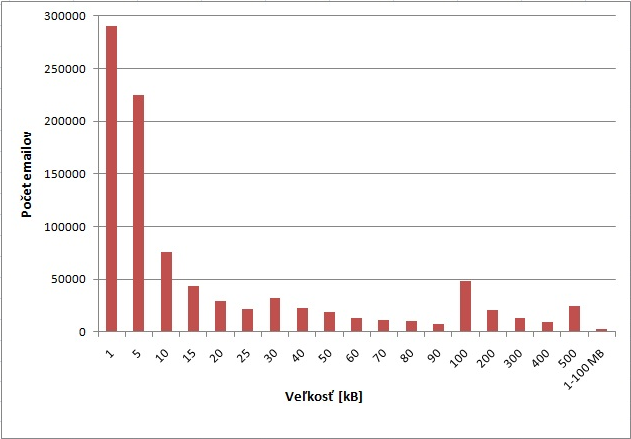
\includegraphics[width=12cm]{./figures/emailsHist.png}
 % topologies802154.png: 722x407 pixel, 72dpi, 25.47x14.36 cm, bb=0 0 722 407
 \caption{Približná distribúcia emailových správ. $\mu = 301\,\mathrm{kB}$, $\sigma = 1.3\,\mathrm{MB}$}
 \label{fig:emailHist}
\end{figure}


\subsubsection*{Export emailov}
Systém musí umožnovať prístup k ľubovoľnému uloženému emailu v jeho pôvodnej podobe poprípadne skupine všetkých emailov patriacej danému užívateľovi (inbox).

\subsubsection*{Vyhľadávanie emailov}
Vyhľadávanie je potrebné realizovať nad všetkými emailovými správami uloženými v systéme, jednotlivo nad správami podľa danej domény a nad správami, ktoré prináležia danému uživateľovi. Požadujeme fultextové vyhľadávanie emailov podľa následujúcich údajov:
%nachádzajúcich sa v obálke, podľa hlavičiek (predmet správy, odosielateľ, príjemca), podľa textu obsiahnutom v tele správy a podľa názvu prílohy.
\begin{itemize}
 \item
  príjemca emailovej správy
 \item
  odosielateľ emailovej správy
 \item
  predmet správy
 \item
  dátum obsiahnutý v emailovej správe
 \item
  identifikátor emailu (\emph{MessageID})
 \item
  názvy príloh a ich veľkosti %TODO aj velkosti?
 \item
  veľkosť emailu
 \item
  vyhľadávanie v tele emailu
\end{itemize}

\newpage
\noindent
Pre administrátorské účely požadujeme vyhľadávanie údajov podľa: %TODO ref na popis email struct
\begin{itemize}
 \item originálny odosielateľ a príjemca
 \item IP adresa odosielateľa
 \item dátum a čas spracovania správy emailovým serverom
\end{itemize}


\subsubsection*{Štatistické údaje}
Nad uloženými dátami požadujeme výpočet štatistík pomocou využitia MapReduce. Pre emaily patriace do danej domény je potrebné spracovať následujúce štatistické ukazateľe:

\begin{itemize}
  \item
  počet emailov označených príznakom spam
  \item
  počet emailov bez príznaku spam
  \item
  celková veľkosť emailov pre danú doménu
  \item
  veľkosť najväčšieho emailu v doméne
  \item 
  celková dĺžka filtrácie emailov v danej doméne %TODO>pod ciaru odkia a co to reprezentuje>doba spracovania emailu pomocou antivírových a antispamových aplikácií
\end{itemize}
\noindent
%TODO: v pigu doriesit statistiky - hodit do zaveru?
Nad celým úložiskom je ďalej potrebné spracovať tieto štatistiky:
\begin{itemize}
  \item
  počet všetkých emailov
  \item 
  počet unikátnych domén
  \item
  počet unikátnych príloh
  %\item
  %počet deduplikácií
\end{itemize}


% \begin{itemize}
%  \item
%   vyhľadávanie emailov podľa údajov tvoriacich obálku, podľa hlavičiek (predmet, odosielateľ, príjemca), podľa textu obsiahnutom v tele správy a podľa názvu prílohy
%  \item
%   prístup koncových užívateľov k archívu, jeho prehľadávanie, export vybraných emailov
%  \item
%   tvorba štatistík (ich konkrétny popis)
%  \item
%   expirácia emailov uložených v databáze po predom určenej dobe
%  \item
%   unikátne ukladanie príloh emailov z dôvodu úspory diskového priestoru
% \end{itemize}

%Emailová správa je štruktúrovaný objekt, časť z našich funkcií systému bude s touto štruktúrou a jej časťami pracovať, rozhodli sme sa, že náš výber noSQL systému zúžime na tie systémy, ktoré využívajú stĺpcový dátový model.



\subsection{Nefunkčné požiadavky}

\subsubsection*{Dostupnosť}
%TODO:ref do slovnicka - def. network partiti
Systém musí byť neustále dostupný (99,9\%), schopný odolávať sieťovým prerušeniam spôsobujúcim nedostupnosť uzlov, úplným zlyhaniam jednotlivých uzlov a umožnovať spracúvať tok pre zápis dát v rozmedzí 10 Mbit až 1 Gbit. Ďalším požiadavkom je aby sa dáta replikovali vo vnútri datacentra na dva uzly a tretia replika bola umiestnená v datacentre, ktoré sa bude nachádzať na geograficky odlišnom mieste. Vyžadujeme aby systém neobsahoval kritický bod výpadku, požadujeme vlastnosť decentralizácie.

\subsubsection*{Rozšíriteľnosť}
%TODO:ref do slovnicka - def. commodity hw
Predpokladáme použitie bežne dostupného spotrebného hardvéru (commodity hardware\footnote{komponenty sú štandardizované, bežne dostupné a ich cenu neurčuje výrobca (IBM, DELL,...) ale trh.}), namiesto superpočítačov. Z dôvodu neustalého nárastu objemu elektronickej pošty, musí systém podporovať horizontálne škálovanie, ktoré bude schopné umožnovať zvýšenie celkovej kapacity dátového úložiska (desiatky petabajtov). Pridávanie nových uzlov do systému umožní zvyšiť celkový vypočetný výkon, ktorý sa využije na spracovanie dát pomocou techniky MapReduce. U distribuovaného databazového systému je nutná podpora replikácie, ktorá zvýši výkonnosť operácií pre čítanie, zápis a vďaka nej nebude potrebné riešiť zalohovanie pomocou externých systémov.

\subsubsection*{Nízkonákladová administrácia}
Prevádzkovanie systému a jeho administrácia by mali byť čo najmenej závislé na zásahu ľudských zdrojov. Detekcia nefunkčných uzlov a automatické rozdeľovanie záťaže sa musí vykonávať automaticky. Pridanie poprípade odobranie nového uzla nesmie ovplyvniť beh celkového systému.

\subsubsection*{Bezpečnosť}
Osoby s oprávnením pre prístup k systému budú schopné manipulovať s jeho celým obsahom. Predpokladáme beh systému v bezpečnom prostredí a nekladieme žiadne požiadavky na uživateľské role v kontexte prístupu k datam.

\subsubsection*{Implementačné požiadavky}
Cieľom je implementácia systému s využitím dostupných open source technologíí. 

%TODO dalsie problemy
\subsubsection*{}
Z analýzy princípov, v predchádzajúcej kapitole, ktoré využívajú relačné databázové syśtémy vyplýva, že použitie týchto systémov nie je vhodné pre riešenie zadefinovaného problému. Medzi základné problémy týchto systémov patrí náročné horizontálne škalovanie, čo negatívne ovplyvňuje primárny požiadavok vysokej dostupnosti. V nasledujúcej kapitole sa budeme zaoberať popisom NoSQL systémov a po ich analýze vyberieme vhodného kandidáta, ktorého použijeme k implementácii prototypu, z dôvodu vyskokej komplexnosti riešeného problému.



%%%%%%%%%%%%%%%%%%%%%%%%%%%%%%%%%%%%%%%%%%%%%%%%%%%%%%%%%%%%%%%%%%%%%%%%%%%%%%%%%%%%%%%%%%%%%%%%%%%%%%%%%%%%%%%%%%%%%%%%%%%%%%%%%%%%%
%%%%%%%%%%%%%%%%%%%%%%%%%%%%%%%%%%%%%%%%%%%%%%%%%%%%%%%%%%%%%%%%%%%%%%%%%%%%%%%%%%%%%%%%%%%%%%%%%%%%%%%%%%%%%%%%%%%%%%%%%%%%%%%%%%%%%
%%%%%%%%%%%%%%%%%%%%%%%%%%%%%%%%%%%%%%%%%%%%%%%%%%%%%%%%%%%%%%%%%%%%%%%%%%%%%%%%%%%%%%%%%%%%%%%%%%%%%%%%%%%%%%%%%%%%%%%%%%%%%%%%%%%%%


\chapter{NoSQL}
\label{chapter:NoSQL}
Názov NoSQL bol prvykrát použitý v roku 1998 ako názov relačnej databáze\footnote{http://www.strozzi.it/cgi-bin/CSA/tw7/I/en\_US/nosql}, ktorej implementácia bola v interpretovaných programovacích jazykoch a neobsahovala dotazovací jazyk SQL. V druhej polovici roku 2009 sa názov NoSQL začal používať v spojení s databázovými systémami, ktoré nepouživajú tradičný relačný model, dotazovací jazyk SQL, sú schopné horizontálneho škálovania, pracujú na spotrebných počítačových systémoch, vyznačujú sa vysokou dostupnosťou a používajú bezschémový dátový model.

Pôvodným cieľom hnutia NoSQL bolo vytvoriť koncept, pre tvorbu moderných databáz, ktoré by boli schopné spracúvať požiadavky neustále sa rozvýjajúcich webových aplikácií. Filozofiou týchto systémov je nesnažiť sa za každú cenu prispôsobovať dáta, ktoré do nich ukladáme relačnému databázovému modelu. Cieľom je vybrať systém, ktorý bude čo najvhodnejšie zodpovedať požiadavkom pre uloženie a spracovanie dát. NoSQL nepopisuje žiaden konkrétny databázový systém, namiesto toho je to obecný názov pre nerelačné (non-relational) databázové systémy, ktoré disponujú odlišnými vlastnosťami a umožnujú prácu s rôznými dátovými modelmi. Medzi ich ďalšie znaky patrí napríklad čiastočná konzistencia, schopnosť spracúvať obrovské objemy dát (PB) a jednoduché programové rozhranie (API). Tieto systémy nepodporujú operáciu databázového spojenia a medzi dátami, ktoré do nich ukladáme je možné vytvárať vzájomné závislosti až na aplikačnej úrovni. Pre tieto databázove systémy ďalej platí, že sú distribuované, automaticky poskytujú replikáciu a rozdeľovanie dát. Jedná sa o relatívne mladé systémy, ktoré sú neustále vo vývoji. Ideou tohto konceptu je riešiť spomínané novo vznikajúce problémy a zároveň koexistovať s relačnými databázovými systémami.

%v pripade relac db sa snazime navrhnut datovy model a nasledne na nom vytvorit vhodne poziadavky v SQL, u tychto systemov vsak plati, ze na zaklade toho ako budu vyzerat dotazy na data namodelujeme datovy model (scheme free)

\section{Dátové modely}

% \section{Dátové modely}
NoSQL systémy delíme na dokumentové, grafové, stĺpcové a systémy s dátovým modelom typu \uv{kľúč-hodnota} (Key-value). V následujúcej časti práce ich stručne popíšeme.

% \subsection{Relačný dátový model}
% %TODO: podla pokorneho opravit ? relacie
% Relačný databázový model reprezentuje dáta pomocou riadkov tabuliek. Tieto riadky reprezentujú relácie, ktoré modelujú závislosti medzi dátami. Popis stĺpcov určuje schému relácie.
% 
% 
% 
% tvorené stĺpcami a ich štruktúra je popísaná schémou. Schéma definuje názvy tabuliek, stĺpcov a podlieha normalizácii aby sa predišlo duplikácii dát. Pre zabezpečenie referenčnej integrity jednotlivých entít sa využívajú cudzie kľúče.
% Každý riadok tabuľky reprezentuje dáta, ktoré sa nazývajú záznamy a tieto sú následne sekvenčne ukladané na pevný disk. Tento model, nazývaný aj ako riadkový, je vhodný pre systémy, u ktorých sú dominantné operácie vykonávajúce zápis. Relačné databázové systémy, využívajúce tento model sú teda optimalizované pre zápis. Pre efektívny prístup k dátam je možné použiť indexy.
% 

% NoSQL systémy delíme na dokumentové, grafové, stĺpcové a systémy s dátovým modelom typu \uv{kľúč-hodnota} (Key-value). V následujúcej časti práce ich stručne popíšeme.

\subsection{Relačný model}
Relačný databázový model reprezentuje dáta pomocou relácií, ktoré tvoria riadky uložené v tabuľkách. Štruktúra týchto záznamov je normalizovaná aby sa predišlo ich duplikácii. Pre zabezpečenie referenčnej integrity jednotlivých entít sa využívajú cudzie kľúče. Tabuľky s popisom názvov stĺpcov a vzťahy medzi nimi nazývame databázovou schémou. Záznamy sú sekvenčne ukladané na pevný disk. Tento model je vhodný pre systémy, u ktorých sú dominantné operácie vykonávajúce zápis. Relačné databázové systémy sú teda optimalizované pre zápis. Pre efektívny prístup k dátam je možné použiť indexy.

%TODO: na vsetky DB ref??
\subsection{Kľúč-hodnota}
%http://ayende.com/Blog/archive/2010/03/29/that-no-sql-thing-keyvalue-stores.aspx


Tento model využíva pre ukládanie dát jednoduchý princíp. Blok dát s ľubovoľnou štruktúrou je v databáze uložený pod názvom kľúča, ktorý je často interne reprezentovaný ako poľe bajtov a môže ním byť napríklad textový reťazec. Databázové systémy využívajúce tento dátový model majú jednoduché programové rozhranie, znázorné na obrázku XY.

\begin{verbatim}
void Put(string kluc, byte[] data);
byte[] Get(string key);
void Remove(string key);
\end{verbatim}


Výhodou tohto modelu je, že databázový systém je možné ľahko škálovať. V tomto prípade prácu so štruktúrou uložených dát zabezpečuje klient, čo umožnuje dosahovať vysokú výkonnosť na strane databázového systému.

Jednou z možných nevýhod v porovaní s relačnými databázovými systémami je, že databázový systém nie je schopný medzi uloženými dátami zachytiť ich vzájomné vzťahy (relácie), čo môže byť jedným z požiadavkov pri tvorbe komplexných modelov. Úložiško typu kľúč-hodnota nevyužíva normalizáciu dát, dáta sú často duplikované, vzťahy a integrita medzi nimi sa riešia až na aplikačnej úrovni. Na obsah vkladaných dát a k nim asociovaným kľúčom sa nedefinujú žiadne obmedzenia.

Medzi databázové systémy využívajúce model kľúč-hodnota patria Amazon Dynamo, Tokyo Cabinet \cite{TODO}, Voldemort \cite{TODO}, Redis \cite{TODO} a iné.

\subsection{Stĺpcovo orientovaný model}
%10.1.1.151.2270.pdf

%obrazok?
%abadiph.pdf

V dnešnej dobe existuje veľký počet aplikácií, u ktorých prevládajú operácie čítania nad zápisom. Patria sem dátové sklady, systémy pre vyťažovanie dát alebo analytické aplikácie pracujúce s obrovským objemom dát. Pre potreby týchto aplikácií a ich reprezentáciu dát je vhodné použiť stĺpcový model \cite{abadi2009column, abadi2009}, ktorý je optimalizovaný pre operácie čítania dát. Data reprezentujúce stĺpce sú uložené na pevnom disku v samostatných a súvislých blokoch. Načítanie dát do pamäti a následná práca s nimi je efektivnejšia ako u riadkových databáz, kde je potrebné načítať celý záznam obsahujúci aj hodnoty stĺpcov, ktoré sú v daný moment irelevantné.

Riadkový model obsahuje v jednom zázname dáta z rôznych domén, čo spôsobuje vyššiu entropiu v porovnaní so stĺpcovým modelom, kde sa predpokláda, že dáta v danom stĺpci pochádzajú z totožnej domény a sú si preto podobné. Táto vlasnosť umožnuje efektívnu komprimáciu dát, ktorá znižuje počet diskových operácií. Nevýdou tohto modelu je zápis dát, ktorý spôsobuje vyššiu záťaž diskových operácií. Pre optimalizáciu operácií vykonavajúcich zápis sa používa dávkový zápis.

% obrazok ?
%\subsubsection*{Stĺpcovo orientovaný model v NoSQL}
%http://ayende.com/Blog/archive/2010/05/14/that-no-sql-thing-column-family-databases.aspx
%Predchodcom tohto nového prístupu k stĺpcovému modelu v NoSQL systémoch je databázový systém Bigtable od spoločnosti Google. Detailnejšie tento model popíšeme v TODO následujúcej kapitole.

%-- a na dáta pozeráme ako na viacdimenzionálnu hešovú-mapu.
%??? obrazok
Tento model využívajú databázové systémy ako Google Bigtable, HBase, Hypertable alebo Cassandra.

\subsection{Dokumentový model}

Dokumentové databázy sú založené na modeli typu kľúč-hodnota. Požiadavkom na ukládané dáta je, že musia byť v tvare, ktorý dokáže spracovať databázový systém. Štruktúra vkládaných dát môže byť určená napríklad pomocou XML, JSON, YAML. Schéma týchto systémov následne umožnuje okrem jednoduchého vyhľadávania pomocou modelu kľúč-hodnota vytvárať s využitím indexov zložitejšie dotazy nad dátami, ktoré sú vyhodnocované na strane databázového systému. 

Medzi databáze reprezentujúce tento typ úložiska patrí napríklad CouchDB a MongoDB.

\subsection{Grafový model}
%http://highscalability.com/neo4j-graph-database-kicks-buttox
%http://blog.neo4j.org/2009/04/current-database-debate-and-graph.html
Tento typ databáz využíva pre prácu s dátami matematickú štruktúru graf. Dáta sú reprezentované pomocou uzlov, hran a ich atribútov. Základným objektom je uzol. Pomocou hrán medzi uzlami modelujeme závislosti, ktoré sú popísané pomocou atribútov. Nad uzlami a hranami sa využíva model kľúč-hodnota. Medzi hlavné výhody patrí možnosť prechádzania týchto štruktúr s využitím známych grafových algoritmov. 

Tento model sa napríklad využíva v aplikáciach sociálnych sieti alebo pre sémantický web. Patria sem databázové systémy Neo4j alebo FlockDB.


\section{Porovnanie NoSQL systémov}
%http://www.rackspace.com/cloud/blog/2009/11/09/nosql-ecosystem/
%http://www.infoq.com/articles/graph-nosql-neo4j


%Systémy NoSQL majú odlišné schopnosti, komplexitu a vďaka tomu ich môžeme použiť pre rôzne účely. V predchádzajúcej sekcii sme vykonali základnú kategorizáciu poďla dátového modelu, ktorý tieto systémy poskytujú a ktorý do istej miery definuje ich vyjadrovaciu silu. V tejto časti popíšeme ďalšie vlastnosti, ktoré nám umožnia užšiu kategorizáciu týchto systémov.
%Tieto dátové modely sú navzájom izomorfné \cite{Web1}. Našim cieľom však nemá byť snaha za každú cenu prispôsobiť dáta k danému modelu. Prítomnosť týchto modelov nám naopak dáva možnosť výberu, ktorý zaručí pre našu aplikáciu 

%Hlavným kritériam pre porovnávanie týchto systémov sú následujúce body:
% kriteria na porovnanie nosql
V dnešnej dobe existuje veľké množstvo NoSQL databázových systémov, ktoré majú odlišné vlasnosti, komplexitu a vďaka tomu ich môžeme použiť pre rôzne účely. Snaha porovnať tieto systémy na globálnej úrovni je nerealizovateľná a často vedie k chybám. Cieľom tejto sekcie je definovať základné body vďaka, ktorým je možné tieto systémy kategorizovať a vrámci danej kategórie porovánať. Tieto zistenia nám následne môžu pomôcť pri výbere vhodného systému, ktorý bude vhodný na riešenie našich požiadavok. Následujúce body patria medzi hlavné kritéria pri porovnávaní týchto systémov:
\begin{enumerate}
 \item
  dátový model
 \item 
  dotazovací model
 \item
  škálovateľnosť
 \item 
  schopnosť odolávať chýbam (failure handling)
 \item
  elastickosť
 \item 
  konzistencia dát
 % prostredie kde operuju / klaud alebo azure?
 \item
  prostredie behu
 \item 
  bezpečnosť 
\end{enumerate}

\subsection{Dátový a dotazovací model}
Dátový model definuje štruktúru, ktorá slúži na ukladanie dát v databázovom systéme. Dotazovací model následne definuje obmedzenia a operácie, ktoré je možné nad uloženými dátami vykonávať. V predchádzajúcej sekcii sme popísali základnú kategorizáciu NoSQL systémov poďla dátového modelu. Dátový a dotazovací model do určitej miery popisuje výkonnosť, komplexnosť a vyjadrovaciu silu databázového systému. Dotazovací model určuje programové rozhranie (API).

Pri výbere vhodného dátového modelu pre aplikáciu je dôležité porozumieť štruktúre dát a definovať operácie, ktoré nad týmito dátami budeme vykonávať. Na základe týchto operácii sa navrhne databázová schéma.

%TODO : priklad ... s deduplikaciou <

\subsection{Škálovateľnosť a schopnosť odolávať chybám}
Tieto vlasnosti kladú na systém požiadavky ako podpora replikácie a rozdeľovanie dát. Distribuované databázové systémy implementujú tieto techniky na systémovej úrovni. V prípade ich podpory, môžeme od systému požadovať:
\begin{itemize}
  \item
  podporu replikcácie medzi geograficky oddelenými dátovými centrami
  \item
  možnosť pridania nového uzlu do distribuovaného databázového systému, bez nutnosti zásahu do aplikácie
\end{itemize}

Počet uzlov, na ktorých sa vykonáva replika dát a konfigurácia databázového systému, ktorá podporuje geograficky oddelené dátové centrá určujú stupeň odolnosti systému voči chybám, medzi ktoré patria porucha uzla alebo sieťové prerušenie.

Častým požiadavkom webových aplikácií, z dôvodu neustáleho nárastu dát, na databázový systém je podpora škálovania s cieľom zvýšenia veľkosti databáze. S neustálym vývojom nových aplikácií musíme zároveň uvažovať potrebu škálovania aj z pohľadu komplexnosti dát \cite{segaran2009beautiful}. Výber dátového modelu môže byť ovplyvnený na základe komplexnosti dát. Obrázok \ref{fig:scalling} zachytáva pozíciu dátových modelov z pohľadu škálovania komplexnosti a veľkosti dát.

%http://blogs.neotechnology.com/emil/2009/11/nosql-scaling-to-size-and-scaling-to-complexity.html

\begin{figure}[h]
 \centering
 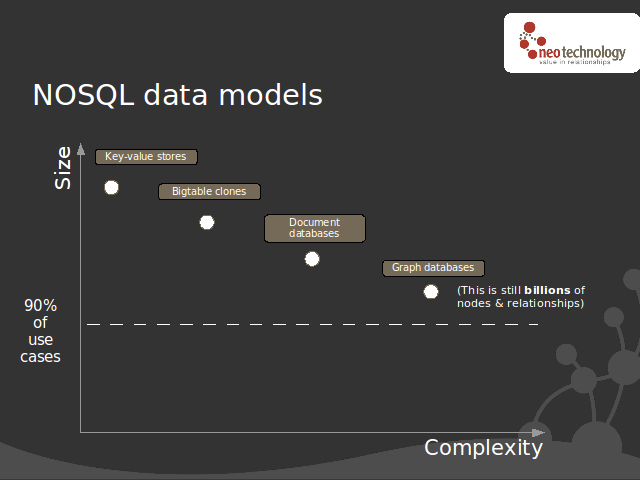
\includegraphics[width=13cm]{./figures/nosqldatamodels.png}
 % topologies802154.png: 722x407 pixel, 72dpi, 25.47x14.36 cm, bb=0 0 722 407
 \caption{Pozícia dátového modelu z pohľadu škálovania podľa veľkosti a komplexnosti. Zdroj: \cite{neo4j}}
 \label{fig:scalling}
\end{figure}
%TODO: http://www.slideshare.net/emileifrem/nosql-overview-neo4j-intro-and-production-example-qcon-london-2010

Dátový model typu kľuč-hodnota a stĺpcovo orientovaný model (Bigtable clones) majú jednoduchú štruktúru, ktorá kladie minimálnu náročnosť v prípade horizontálneho škálovania. Nevýhodou tohto prístupu je naopak to, že všetká práca s dátami a ich štruktúrou sa prenáša do vyšších vrstiev, o ktoré sa musí starať programátor. Naopak dokumentový a grafový model poskytuje bohatšiu štruktúru na prácu s dátami, ktorá spôsobuje komplikovanejšie škálovanie vhľadom k veľkosťi dát. Podľa odhadov spoločnosti Neotechnology\footnote{http://neotechnology.com/} až 90\% aplikáci, v prípade že sa nejedná o projekty spoločností Google, Amazon atď., spadá do rozmedzia kde sa veľkosť záznamov pohybuje rádovo v miliardách. Za zmienku stojí fakt, že aj napriek tomu, že tieto dátové modely sú si navzájom izomorfné, vhodnosť ich použitia závisí na konkrétnom príklade a požiadavkoch na aplikáciu. 

%one size fits all?
\subsection{Elastickosť}
% Vďaka horizontálnemu škálovaniu sa snažime o zýšenie kapacity a dostupnosti dátového úložiska. 
Elastickosť škálovania popisuje ako sa daný systém dokáže vysporiadať s pridaním alebo odobraním uzla. Určuje do akej miery je v tomto prípade potrebný manuálny zásah pre rovnomerné rozloženie záťaže, prípadná potreba reštartovania systému alebo zmena v užívateľskej aplikácii. Ideálne by pridávanie nových uzlov do systému malo zabezpečiť lineárne zvyšovanie výkonu u operácií ako je čítanie alebo zapisovanie dát.


\subsection{Konzistencia dát}
Poďla teórie CAP platí, že v prípade výskytu sieťových prerušení, ktorých prítomnosť v prostredí distribuovaných databázových systémov je prirodzená, nie je možné súčasne zaručiť vlasnosť konzistencie a dostupnosti. NoSQL systémy preto môžeme rozdeliť podľa tohto modelu do dvoch skupín, ktoré znázorňuje obrázok \ref{fig:scalling}. Umiestnenie niektorých datázových systémov sa môže meniť na základe ich konfigurácie. 

\begin{figure}[h]
 \centering
 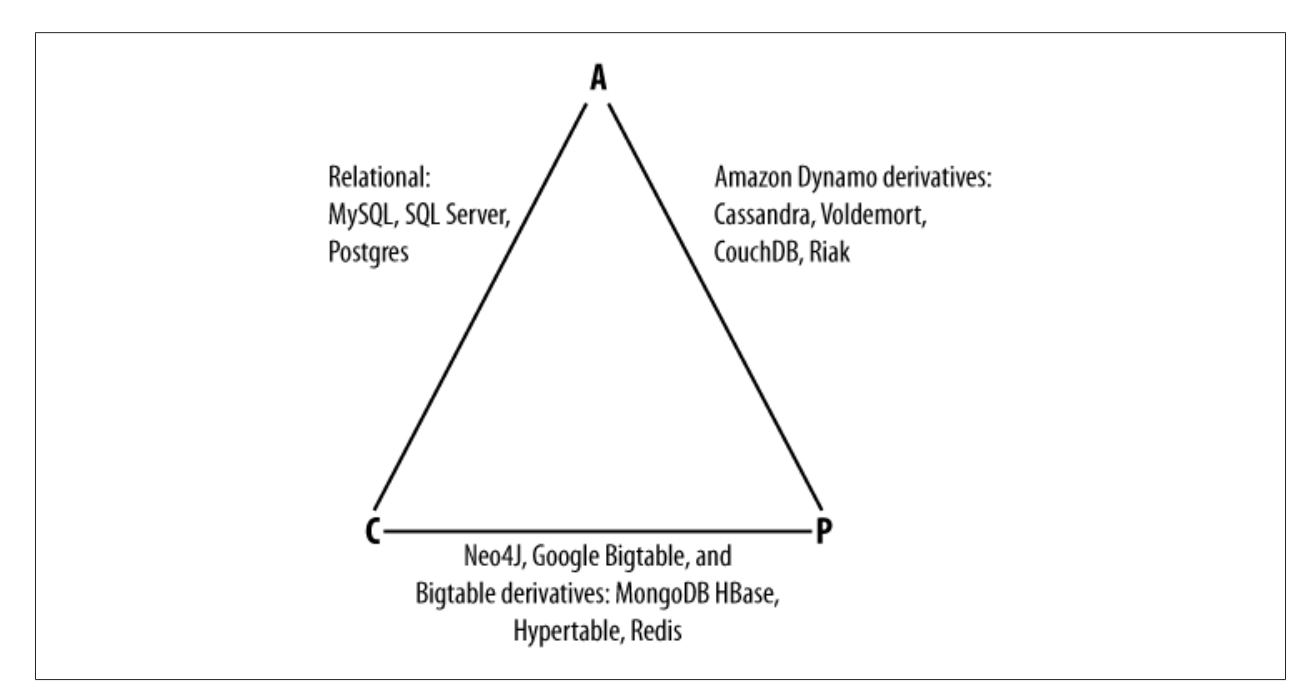
\includegraphics[width=13cm]{./figures/capDatabases.png}
 % topologies802154.png: 722x407 pixel, 72dpi, 25.47x14.36 cm, bb=0 0 722 407
 \caption{Rozdelenie databázových systémov podľa CAP}
 \label{fig:scalling}
\end{figure}


\subsection{Prostredie behu}
NoSQL systémy ďalej delíme  podľa prostredia, v ktorom pracujú. Väčšina týchto open source systémov umožnuje ich nasadenie do vlastného prostredia teda privátnych cloudov alebo do verejného cloudového riešenia EC2 od spoločnosti Amazon. Mezdi tieto systémy patria napríklad Cassandra, HBase, Riak, Voldemort. Databázové systémy Amazon SimpleDB, Microsoft Azure SQL, Yahoo! YQL alebo Google App Engine sú poskytované ako komplexné cloudové riešenie. Rozhranie pre prácu s dátami a funkčnosť perzistentného úložiska zabezpečujú poskytovatelia týchto systémov.



\subsection{Bezpečnosť}
Distribuovaný databázový systém je možné nasadiť do cloudu. V prípade, použitia verejných cloudov môže hroziť nebezpečenstvo zneužitia dát treťou stranou a preto je potrebné aplikovať bezpečnostné mechanizmy. Pri nasadení systému do privátneho cloudu zasa môžeme požadovať viacero úrovní ochrany pre prístup k dátam. Systémy NoSQL disponujú minimálnymi prvkami pre zaručenie autentizácie a autorizácie. Mnoho systémov tieto mechanizmy vôbec neimplementuje poprípade ich implementácia je v začiatkoch.

%TODO
%\subsection{Bezpečnosť}

%Snaha o globlálne výkonostné testy NoSQL systémov by viedla k porovnávaniu \uv{jabĺk s hruškami}.
%V následujúcej sekcii využijeme Yahoo! Cloud Serving Benchmark pre porovnanie nami vybraných kandidátov.

\section{Výber NoSQL systémov}
%http://themindstorms.blogspot.com/2009/05/quick-reference-to-alternative-data.html
%http://www.metabrew.com/article/anti-rdbms-a-list-of-distributed-key-value-stores

V predchádzajúcej sekcii sme tieto distribuované databázové systémy rozdelili do štyroch hlavných kategórií na základe ich dátového modelu, ktorý je jedným z kľúčových faktorov pri výbere vhodného kandidáta podľa požiadavkov cieľovej aplikácie. Detailný popis a výkonnostné porovnanie NoSQL systémov, ktoré reprezentujú jednotlivé kategórie by boli nad rámec tejto práce. Paralelne s touto prácou vzniká diplomová práca, ktorá rieši podobný problém s využitím dokumentových databázových systémov  \cite{barina}, preto túto kategóriu pri výbere vynecháme.

%TODO referencie
Podľa analýzy požiadavkov na našu aplikáciu, ktoré sme popísali v predchádzajúcej kapitole nie je vhodné použitie databázových systémov s grafovým modelom a modelom typu kľúč-hodnota. Systémy s grafovým modelom sú určené na odlišnú úlohu problémov. V prípade použitia systémov s dátovým modelom kľúč-hodnota by sme komplexnosť riešenej úlohy preniesli na úroveň klienta. Našim požiadavkom najlepšie vyhovuje stĺpcovo orientovaný model, ktorý využijeme v návrhu našej aplikácie. Hlavnou výhodou je, že tento model u systémov NoSQL nestanovuje žiadnu schému na dáta, ktoré budeme do systému vkládať, počet sĺpcov závisí od vstupných dát a ich počet je ľubovoľný. Pre potreby nášho riešenia preto použijeme stĺpcovo orientovaný NoSQL systém.

\subsection*{Stĺpcovo orientované NoSQL systémy}
%TODO referencie
V tejto časti sa zameriame na vzájomné porovnanie systémov, ktoré poskytujú stĺpcovo orientovaný model. Medzi tieto open source systémy patria HBase, Cassandra a Hypertable. Napriek totožnému dátovemu modelu sú tieto systémy založené na rôznych architektonických princípoch a disponujú čiastočne odlišnými vlasnosťami. Tabuľka \ref{tab:Nosql} zobrazuje stručný prehľad vlasností, na ktoré sme sa zamerali pri výbere víťaznej dvojice.


% \begin{table}[hp]
% \begin{center}
%     \begin{tabular}{|l|l|l|l|}
% 	\hline 
% 	\multirow{2}{*}{Vlastnosti} & \multicolumn{3}{|c|}{Databázový systém}  \\
% 	\hline & HBase & Cassandra & Hypertable \\  \hline
% 
%         Distribuovaný systém	& áno  & áno & áno \\ \hline 
%         Architektúra		& Bigtable \footnote{lala} & Dynamo & Bigtable \\ \hline
% 	Klient 			& Thrift, REST  & Thrift, Avro & Thrift, C++ \\ \hline
%         Perzistentné úložisko	& HDFS, AS3, KFS  & LSS\footnote{lokálny súborový systém} & HDFS, KFS, LSS \\ \hline
%         SPOF \footnote{SPOF - uzol, ktorého nedostupnosť spôsobí nedostupnosť celého systému}	& áno  & nie & - \\ \hline
% 	Podpora viacerých datacentier & áno  & áno & áno \\ \hline
% 	Automatické rodeľovanie dát 	& áno  & áno & áno \\ \hline
%         Replikácia 		& áno  & áno & áno \\ \hline
% 	Konzistencia 		& CP  & AP & CP \\ \hline
% 	Programovací jazyk 	& Java  & Java & C++ \\ \hline
% 	MapReduce 		& áno  & áno & áno \\ \hline
% 	Dokumentácia		& +  & +  & - \\ \hline
% 	Komunita 		& +  & +  & - \\ \hline
%     \end{tabular}
% \end{center}
% \caption{Priepustnosť pri zápise dát na HDFS}
% \label{tab:Nosql}
% \end{table}

{\centering\par\bigskip
\begin{tabular}{l@{\hspace{2.5em}}lll}\toprule
Vlastnosť & \multicolumn{3}{c}{Databázový systém} \\
			& \multicolumn{1}{l}{HBase} & \multicolumn{1}{l}{Cassandra} & \multicolumn{1}{l}{Hypertable}\\\midrule\addlinespace

Distribuovaný systém	& áno  & áno & áno 				\\\addlinespace
Architektúra		& Bigtable  & Dynamo & Bigtable	\\\addlinespace
Klient 			& Thrift, REST  & Thrift, Avro & Thrift, C++ 	\\\addlinespace
Perzistentné úložisko	& HDFS, AS3, KFS  & LSS\footnote{lokálny súborový systém} & HDFS, KFS, LSS		\\\addlinespace
SPOF	& áno  & nie & -\footnote{zalezi na type uloziska} 	\\\addlinespace
Podpora viacerých datacentier & áno  & áno & áno 			\\\addlinespace
Automatické rozdeľovanie dát 	& áno  & áno & áno 			\\\addlinespace
Replikácia 		& áno  & áno & áno 				\\\addlinespace
Konzistencia 		& CP  & voliteľná & CP 				\\\addlinespace
Kompresia dát		& LZO, GZIP  & nie & LZO, ZLIB 				\\\addlinespace
Programovací jazyk 	& Java  & Java & C++ 				\\\addlinespace
MapReduce 		& áno  & áno & áno 				\\\addlinespace
Indexy		 	& -  & +  & - 					\\\addlinespace
Dokumentácia		& +  & ++  & - 					\\\addlinespace
Komunita 		& +  & +  & - 					\\\addlinespace\bottomrule

\end{tabular}\\}
\captionof{table}{Stručný prehľad vlasností stĺpcovo orientovaných systémov NoSQL}\label{tab:Nosql}
\par\bigskip



Zo stručného prehľadu v tabuľke je vidieť, že systémy obsahujú množstvo spoločných vlastností. Pri výbere sme zohľadnili aj ich praktické využitie spoločnosťami globálne pôsobiacimi na IT trhu. Napríklad systém Cassandra je používaný spoločnosťou Facebook v aplikácii pre vyhľadávanie a uchovávanie súkromnej pošty. Ďalšími dôležitými požiadavkami pre výber boli podpora komunity a kvalita dokumentácie. U systému Cassandra zohrala pri výbere hlavnú rolu decentralizácia a možnosť voľby medzi konzistenciou a dostupnosťou. Zo zvolených kandidátov sme vybrali systém HBase a Cassandra. Dôvodom prečo sme zavrhli systém Hypertable je nedostačujúca dokumentácia, málo aktívna komunita a v čase výberu sa nachádzal vo verzii alfa. V následujúcich dvoch kapitolách detailne popíšeme oba systémy.

Počas písania tejto práce bol uvoľnený ďalší open source distribuovaný databázový systém implementujúci model Bigtable pod názvom Cloudata\footnote{http://www.cloudata.org}, ktorý sme už do naše práce nezahrnuli.
%TODO no transactions
%C = rack aware + sec indices, 
%hdfs SPOF



%%%%%%%%%%%%%%%%%%%%%%%%%%%%%%%%%%%%%%%%%%%%%%%%%%%%%%%%%%%%%%%%%%%%%%%%%%%%%%%%%%%%%%%%%%%%%%%%%%%%%%%%%%%%%%%%%%%%%%%%%%%%%%%%%%%%%
%%%%%%%%%%%%%%%%%%%%%%%%%%%%%%%%%%%%%%%%%%%%%%%%%%%%%%%%%%%%%%%%%%%%%%%%%%%%%%%%%%%%%%%%%%%%%%%%%%%%%%%%%%%%%%%%%%%%%%%%%%%%%%%%%%%%%
%%%%%%%%%%%%%%%%%%%%%%%%%%%%%%%%%%%%%%%%%%%%%%%%%%%%%%%%%%%%%%%%%%%%%%%%%%%%%%%%%%%%%%%%%%%%%%%%%%%%%%%%%%%%%%%%%%%%%%%%%%%%%%%%%%%%%

\chapter{Cassandra}
%TODO: zadefinovat spotrebny pocitac
%TODO: podla clanku google zadefinovat ze poruchovost HW je taka a taka

%TODO : popisat strucne MVCC

Distribuovaný databázový systém Cassandra bol vytvorený pre interné účely spoločnosti Facebook v roku 2007. Cassandra slúžila na vyhľadávanie v súkromnej pošte a poskytovala úložisko pre indexy vytvárané nad týmito dátami. Od systému sa predpokládalo, že bude obsluhovať miliardy zápisov denne, podporovať škálovanie podľa narástajúceho počtu použivateľov, umožnovať beh na spotrebných počítačoch a podporovať replikáciu medzi geograficky oddelenými dátovými centrami. Ďalším požiadavkom bola vysoká dostupnosť, aby chyba žiadného uzlu nespôsobila celkovú nedostupnosť systému. Cassandra je decentralizovaný systém, kde každý uzol vykonáva tie isté operácie. V roku 2008 bola zverejnená ako open source projekt a je neustále vyvíjaná mnohými spoločnosťami a vývojármi. Tento systém využíva architektonické princípy distribuovaného databázového systému Dynamo \cite{decandia2007dynamo} od spoločnosti Amazon a dátový model prevzal od distribuovaného databázového systému Bigtable vytvoreného spoločnosťou Google. V následujúcom texte popíšeme hlavne princípy, na ktorých je tento systém založený.


\section{Dátový model}
Cassandra k dátovému modelu systému Bigtable pridala štruktúru pod názvom \emph{\uv{super stĺpec}} (Super column). Základnou jednotkou dátového modelu je stĺpec. Stĺpec je tvorený názvom, hodnotou a časovým odtlačkom, ktorý využíva Cassandra pri riešení konfliktov súbežného zápisu. Skupina stĺpcov je identifikovná pomocou unikátneho kľúča a predstavuje riadok, počet a názvy stĺpcov nie je potrebné vopred definovať. Zoradené riadky podľa hodnoty kľučov a v nich zoradené stĺpce obaľuje štruktúra pod názvom \emph{\uv{rodina stĺpcov}} (Column family). Kľúče interne reprezentované ako reťazec znakov sú zároveň zotriedené. Názvy stĺpcov možu byť viacerých typov ako napríklad \emph{ASCII}, \emph{UTF-8}, bajtové pole a iné, podľa ktorých sú zotriedené. Je možné implementovať vlastnú metódu pre triedenie. Riadky obsiahnuté v jednej rodine stĺpcov sú na pevnom disku fyzicky umiestnené v jednom súbore typu \emph{SSTable}. Je vhodné do rodiny stĺpcov ukládať relevantné záznamy, ku ktorým budeme pristupovať spoločne, čim sa vyhneme nadbytočným diskovým operáciam. V rámci jednej repliky sú operácie nad stĺpcami atomické. Operácie nad riadkom nevyužívajú zamykanie. Voliteľným príznakom, ktorý môžeme u stĺpca nastaviť je parameter TTL (Time to live), ktorý po uplynutí časového intervalu označí dáta príznakom pre zmazanie.

Štruktúra super stĺpec je špecialny typ stĺpca, ktorý je tvorenými obyčajnými stĺpcami. Stĺpec typu super má názov a jeho hodnota je tvorená zoznamom názvov obyčajných stĺpcov. Super stĺpce obaľuje štruktúra pod názvom \emph{\uv{super-rodina stĺpcov}} (Super column family). \emph{Keyspace} združuje rodiny a super-rodiny stĺpcov. Definuje faktor a metódu replikácie, ktorá môže byť závislá poprípade nezávislá na sieťovej topológii. Na keyspace sa môžeme pozerať ako na databázu a rodiny stĺpcov môžeme prirovnať k tabuľkám v relačných databázových systémoch.

Aktuálna verzia Cassandry definuje maximálnu veľkosť dát 2 GB, ktoré je možné uložit do jedného stĺpca a stanovuje limit dve miliardy pre maximálny počet stĺpcov tvoriacih riadok.

%TODO: obrazok


\section{Rozdeľovanie dát}
%vuh1093.pdf
Kľúčovým požiadavkom systému Cassandra je jeho schopnosť horizontálneho škálovania, čo vyžaduje pridávanie nových uzlov. Tento požiadavok vyžaduje mechanizmus, ktorý zabezpečí automatické rozdeľovanie dát medzi uzlami systému. Uvažujme príklad, kde máme k dispozícii jeden server obsahujúci veľké množstvo objektov, ku ktorým pristupujú klienti. Medzi server a klientov vložíme vrstvu kešovacích systémov, kde každý z týchto systémov bude zodpovedný za prístup k časti objektov nachádzajúcich sa na serveroch. Klient musí byť schopný určiť na základe hľadaného objektu, ku ktorém kešovaciemu systému. Predpokladajme, že klientom zabezpečíme výber jednotlivých kešovacím systémom pomocou lineárnej hašovacej funkcie ${y = ax + b (mod\,\ p)}$, kde $p$ je počet kešovacích systémov. Pridanie nového kešovacieho systému alebo jeho zlyhanie bude mať katastrofálny dopad na funkčnosť systému. V prípade zmeny hodnoty $p$, bude každá položka odpovedať novej a zároveň chybnej lokácii. Tento problém rieši elegantne technika pod názvom \emph{\uv{úplné hašovanie}} (Consistent hashing) \cite{Karger:1997:CHR:258533.258660}, ktorá sa využíva v distribuovaných systémoch pre určenie pozície pre prístup k distribuovaným hašovacími tabuľkami a využíva ju systém Cassandra.

Výstup hašovacej funkcie MD5 je reprezentovaný pomocou \uv{kruhu}, kde v smere hodinových ručičiek postupujeme od minimálnej hodnoty hašovacej funkcie \textit{0} k maximálnej ${2^{127}}$. Každý uzlol v systéme má pridelenú hodnotu z tohoto rozsahu, ktorá určí jeho jednoznačnú pozíciu. Identifikácia uzlu v systéme, na ktorý sa uložia dáta reprezentované hodnotou kľúča sa vykoná aplikáciou hašovacej funkcie na dáta reprezentujúce kľúč. Na základe tejto hodnoty je jednoznačne určená pozícia v kruhu a v smere hodinových ručiek je vyhľadaný najbližší uzol, ktorému dáta prináležia. Výhodou tejto metódy je, že každý uzol je zodpovedný za hodnotu kľúčov, ktorých poloha sa nachádza medzi ním a jeho predchodcom. V prípade pridania nového uzlu alebo jeho odobratia, sa zmena mapovania kľúčov v kruhu prejaví len u jeho susedov. Táto technika prináša výhody, medzi ktoré patrí rovnomerná distribúcia dát a vyváženie záťaže. Dynamo tento problém rieši spôsobom kde každý uzol je zodpovedný za viacero pozícií na kruhu, takzvané virtuálne pozície. Cassandra využíva vlastné mechanizmy na monitorovanie záťaže uzlov a automaticky presúva ich pozície v kruh. Zároveň je možné explicitne stanoviť polohu každého uzla v kruhu pomocou zadania jeho identifikátora. Tento spôsob je vhodný v prípade, ak vieme predom určiť koľko uzlov bude systém obsahovať. V prípade zvyšovania počtu uzlov je možné tieto identifikátory zmeniť za behu systému. Identifikátor polohy uzlov je možné určiť pomocou následujúceho programu v jazyku Python, kde K je počet uzlov v systéme.

\begin{verbatim}
def tokens(n):
  r = []
  for x in xrange(n):
    r.append(2**127 / n * x)
  return r

print tokens(K)
\end{verbatim}


%TODO Obrazok kruhu


\section{Replikácia}

%S úplným hašovaním úzko súvisý replikácia, ktorá zabezpečuje vysokú dostupnosť a odolnosť dát proti ich stráte (Durability). 
S úplným hašovaním úzko súvisý replikácia. Každá dátová jednotka vložená do systému je replikovaná na N uzlov, kde počet N je voliteľne nastaviteľný pre daný keyspace. Každý uzol sa v prípade replikácie N > 1 stáva koordinátorom, ktorý je zodpovedný za replikáciu dát, ktorých kľúč spadá do jeho rozsahu. Počas operácie zápisu koordinátor replikuje dáta na ďalších N - 1 uzlov. Cassandra podporuje viacero spôsobov pre umiestňovanie replík.

\subsection*{Jednoduchá stratégia}

Táto stratégia umiestňuje replikú dát bez ohľadu na umiestnenie uzlov (serverov) v datacentre. Primárnu repliku spravuje uzol, do ktorého rozsahu spadajú ukladané dáta a ostanté repliky sú uložené na N - 1 susedov v smere hodinových ručičiek. Z toho vyplýva, že každý uzol je zodpovendný za dáta, ktorých kľúče spadajú do jeho rozsahu a súčasne dáta, ktoré spravuje jeho N predchodcov.

\subsection*{Sieťová stratégia}

Pri tejto metóde a úrovni replikácie s hodnotou aspoň tri, je systém schopný zabezpečiť umiestnenie dvoch replík v rozdielnych \emph{\uv{rackoch}}\footnote{TODO popis rack} vrámci jedného datacentra. Tretia replika môže byť umiestnená do geograficky oddeleného datacentra. Táto stratégia je výhodna v prípade ak chceme použiť časť serverov na výpočty pomocou MapReduce a zvyšné dve repliky budú slúžiť na obsluhu reálnej prevádzky.

\section{Členstvo uzlov v systéme}

Distribuovaný systém musí byť schopný odolávať chybám ako porucha uzlov alebo sieťové prerušenia. Decentralizácia a detekcia chýb využíva mechanizmy založené na \emph{gosship protokoloch} \cite{ganesh2003peer}. Tieto protokoly slúžia pre vzájomnú komunikáciu uzlov vymnieňajúcich si navzájom doležité informácie o svojom stave. Periodicky v sekundových intervaloch každý uzol kontaktuje náhodne vybraný uzol, kde si overí či je tento uzol dostupný. Detekcia nedostupnosti uzla je realizovaná algoritmom s názvom Accrual Failure Detector \cite{hayashibara2004}.

Pridávanie novýchu uzlov, presun uzlov v rámci kruhu sa taktiež dejú pomocou Gosship protokolu, ktorý ďalej zabezpečuje, že každý uzol obsahuje informácie o tom, ktorý uzol je zodpovedný za daný rozsah kľúčov v kruhu. Ak sa vykonáva operácia čítania alebo zápisu dát na uzol, ktorý nie je zodpovedný za tento kľúč, dáta sú automaticky preposlané na správny uzol, ktorého výber je zabezpečený s časovou zložitosťou \textit{O(1)}.


\section{Zápis dát}
Tento systém bol primárne navrhnutý tak aby spracúval vysoký tok dát pre zápis. Ak uzol obrží požiadaok pre zápis, dáta sú zapísané do štruktúry pod názvom \emph{Commitlog}, ktorá je uložená na lokálnom súborovom systéme a zabezpečuje trvácnosť dát. Zápis do tejto štruktúry je vykonaný sekvenčne, čo umožnuje dosiahnúť vysokú priepusnosť bez nutnosti vystavovania diskových hlavičiek (disk seek operations). Dáta sú následne zoradené a nahrané do štruktúry pod názvom \emph{Memtable}, ktorej obsah je uložený v operačnej pamati. V prípade, že by tento zápis zlyhal alebo by došlo k neočakávanému pádu inštancie Cassandry obnovenie obsahu týchto štruktúr je možné vďaka Commitlogu. Po dosiahnutí predom stanovej hodnoty, ktorá určuje maximálny počet dát uložených v Memtable sú tieto štruktúry zapísané do súborov pod názvom \emph{SSTable} (Sorted String Tables), ktorých obsah je zoradený podľa hodnoty kľúčov a nie je možné ich modifikovať. Súbory SSTables sa zlievajú (merge sort) v pravidelných intervaloch na pozadí a táto operácia je neblokujúca. Počas zlievania SSTables dochádza k odstraňovaniu dát určených na vymazanie a generovaniu nových indexov. Indexy slúžia na rýchly prístup k dátam uloženým v SSTable. Zároveň sa generujú štruktúry pod názvom \emph{Bloom filters}\footnote{http://en.wikipedia.org/wiki/Bloom\_filter}, ktoré sa využívajú pri čítaní dát. Požiadavok pre zápis dát je možné zaslať na ľubovoľný uzol v klastri.

%sstable data,index,filter?
%http://wiki.apache.org/cassandra/ArchitectureOverview

\section{Čítanie dát}
V prípade požiadavku na načitanie dát, sa požadované dáta najprv hľadajú v štruktúrach Memtable. Ak sa dané data nenachádzajú v operačnej pamati, vyhľadávanie sa uskutočnuje podľa kľúča v súboroch SSTable. Kedže snahou systému, je čo najefektívnejšie vyhľadávanie, využívajú sa bloom filtre. Bloom filtre sú nedeterministické algoritmy, ktoré dokážu otestovať či hľadaný prvok patrí do množiny a generujú len falošné pozitíva. Pomocou nich je možné priradiť kľúče uložené v súboroch SSTables do bitových polí, ktoré je možné uchovať v operačnej pamati. Vďaka tomu sa výrazne redukuje prístup na disk. Požiadavok pre čítanie dát možeme zaslať na ľubovoľný uzol.

\section{Zmazanie dát}
Počas vykonania operácie reprezentujúcej zmazanie dát sa tieto dáta nevymažú okamžite. Namiesto toho sa vykoná operácia, ktorá dané dáta označkuje príznakom pod názvom \emph{tombstone}. Po uplynutí doby, ktorá je štandardne nastavená na desať dní, sa tieto dáta odstránia pri procese zlievajúcom súbory SSTables.
 

\section{Konzistencia}

Konzistencia systému je maximálne konfigurovateľná a využíva princípy techník založených na protokoch kvóra. Klient určuje hodnotu R, ktorá stanovuje počet replík pre čítanie dát. Operácia je úspešná v prípade dostupnosti týchto replík. To samé platí pre zápis dát, kde počet replík je určený parametrom W. Ak je splnený vzťah R + W > N, kde N je počet replík tak výsledok operácie spĺňa definíciu silnej konzistencie, naopak v prípade vzťahu R + W < N, sa jedná o čiastočnú konzistenciu čím zaručíme vysokú dostupnosť.


\section{Perzistentné úložisko}

Cassandra využíva ako perzistentné úložisko dát lokálny súborový systém.


\section{Bezpečnosť}

Implicitne Cassandra nevyužíva žiadne prvky zabezpečujúce bezpečnostné mechanizmy. K dispozícii je modul, ktorý umožnuje nastavenie auntentizácie na úrovni Keyspace-u pomocou textových hesiel alebo ich MD5 odtlačkov. Obmedzovanie prístupu k datám je preto potrebné zabezpečiť na aplikačnej úrovni.

%%%%%


%obmedzenie MYSQL = +papier 5
%mysqlscalling and high avail.pdf -

% 
% Musime predpokladat ze zlyhania v tak velkej infrastrukture su bezna vec a nie ojedinela zalezitost = HW a siet zlyhania
% Zapis nie je nikdy rejectnuty(ani v pripade hw poruchy ani v pripade concurent writes),  z tho odovodu je to alway writtable system = co ale implikuje ze konflikty sa riesia pocas operacie READ
%   riesenie konfliktu na strane db vyuziva jednoduche techniky = last write win, kdezto na strane klienta napriklad mozeme pouzit merge na 2 rozne verzie dat (nakupny kosik)
% bigtable = multi dimensional sorted map
% Zero hop DHS = kazdy uzol obsahuje dostatok informacii na priame presmerovanie poziadavku na cielovy uzol 
% 
% kluc je array of bytes na neho sa aplikuje mdť hash ktory vygeneruje +ľábit identifikator na zaklade ktore sa urci uzol kde budu ulozene data pre dany kluc
% 
% partitioning = consistent hashing = najvacsia hodnota has funkcie v spojeni s najnizsou (0) vytvori kruh na ktory sa umiestnia jednotlive uzly.... data sa potom podla md5(key) umiestnia na dany uzol (v smere hod ruciciek ktoreho  pozicia ja vacsia ako pozicia md5(kluca) Kazdy uzol je takto zodpovedny za svoj region (uzol => predchodca) ... vyhodou konzistent hashovania je ze havaria/pridanie noveho uzla ovplyvňuje len susedov. Tento koncept obsahuje viacero nedostatkov ako napriklad nerovnomerna distribucia zataze.... 
% preto sa aplikuje upraveny consistent hasing a to tak ze kazdy uzol obsahuje viacero virtualnych pozicii na ringu
% 
% 
% Replikacia zabezpecuje hlavne dostupnost a stalost dat {durability}
% 
% 214: W a R impact object availability durability and consistency 
% N R W - 3,2,2 podla dynamo paper {215}
% 
% distirbucia klucov pri malej zatazi - horsie to loadbaloncovalo ako pri velkej zatazi  215
% 209 tabulka + obrazok
% 
% diskusia nad n,r,w 214
% 
% 
% 
% 
% detekcia konfliktov pri upgrade pomocou vector clock - ale kedze mi len WRITE nezaujima nas to
% v pripade ze preda dany stlpec nemame hodnotu nic sa nikam nezapisuje
% 
% 
% kapitola impl -- v pripade ze nejaka polozka neexistuje nic sa nedeje ... neukladame ... handlujeme na strane klienta
% %Rodina stlpcov - last 100 emails , je automaticky zotriedena podla datumu, co podporuje samotna Cassandra.
% Hardware failure is the norm rather than the exception.

\chapter{HBase}
% podla porovnania vybereme 2 a tie dosledne popiseme 
% dovod preco sme vybrali column.familly - graf = komplexnost problemu narast data = a podla neho ze nepotrebujem key-value - zlozita praca so strukt. datami...  a popis 2 vybranych
V úvode tejto kapitoly stručne popíšeme distribuovaný súborový systém, ktorý je súčasťou projektu Hadoop a zároveň slúži ako perzistentné úložisko pre distribuovanú databázu HBase. Následne popíšeme základné princípy fungovania tohoto databázového systému.

\section*{Hadoop}
%shvachko.pdf

Hadoop\footnote{http://hadoop.apache.org/} je open source projekt vytvorený v programovacom jazyku Java, ktorý tvorý distribuovaný súborový systém Hadoop Distributed Filesystem (HDFS) a framework MapReduce pre spracúvanie objemu dát v desiatkách PB \cite{Thusoo:2010:DWA:1807167.1807278}. Medzi hlavné vlastnosti tohoto systému patria vysoká dostupnosť, škálovateľnosť a distribuovaný výpočet. Architektúra HDFS vychádza z princípov distribuovaného súborového systému Google File System (GFS) \cite{Ghemawat:2003:GFS:945445.945450} a pôvod frameworku MapReduce \cite{Dean:2008:MSD:1327452.1327492} pochádza taktiež od spoločnosti Google.

 
%kto ho pouziva a na ake typy appl


Súborový systém využíva architektúru master-slave. HDFS predpokláda prácu so súbormi rádovo v desiatkách gigabajtov, ktoré sú interne reprezentované dátovými blokmi o štandardnej veľkosti 65 MB. Informácie o priradení blokov k súborom a ich umiestnenie na uzloch typu slave sú reprezentované pomocou metadát. Tieto metadáta sú uložené v operačnej pamäti uzla typu master, ktorý sa nazývana \emph{Namenode}. Uzly slave pod názvom \emph{Datanode} slúžia ako fyzické úložisko dátových blokov, ktoré sú zároveň na týchto uzloch replikované. Štandardne je nastavená úroveň replikácie na hodnotu tri,
každý blok je v systéme uložený trikrát.

Predtým ako klient vykoná operáciu zápisu alebo čítania dát, tak kontaktuje uzol Namenode, ktorý mu poskytne informácie, na ktorých uzloch sa nachádzajú bloky reprezentujúce súbor a dátová komunikácia následne prebehne medzi klientom a uzlami typu Datanode. HDFS je optimalizovaný pre jednorázový zápis dát a ich následné mnohonásobné čítanie.

%TODO popisat format metadat ???

Hlavným nedostatkom tejto infraštruktúry je fakt, že uzlol Namenode tvorí kritický bod výpadku, v prípade jeho nedostupnosti nie je možné pracovať s HDFS. Prípadná strata alebo poškodenie dát na tomto uzle spôsobí totálne zlyhanie súborového systému bez možnosti jeho obnovy. Súborový systém nie je vhodný pre ukladanie veľkého počtu malých súborov.
Uzol Namenode alokuje pre objekt typu blok a objekt typu súbor 300 B metadát. V prípade uloženia súboru, ktorý nepresahuje veľkosť jedného bloku je potrebné alokovať 300 B dát. Ak uložíme 10,000,000 takýchto súborov veľkosť metadát, ktoré udržiava Namenode v operačnej pamati zaberie 3 GB. Celkový počet uložených súborov je obmedzený veľkosťou operačnej pamati RAM, ktorou disponuje uzol Namenode.

Z týchto pozorovaní vyplýva fakt, že distribuovaný súborový systém HDFS nemá praktické využitie ako úložisko dát slúžiace k archivácii emailových správ, pre ktoré sme zadefinovali požiadavky v tretej kapitole. %TODO:REF
% 
% SYNC!!! a zapis pipeline style  page 69 hadoop book
% 
% Decisions related to the replication of blocks are always taken
% by NameNode, which receives regularly from each DataNode
% in the cluster Heartbeat information and the proportion
% between the blocks used. The information about a file has the
% form [5]:

%NameNode (File_name,Id_blocs, ...)
%replica_numbers, For exemple the next information:
%/path/part-0,r:2,{1,3},...
%/path/part-0,r:3,{2,6,34},..
% means that part-0 is stored with 2 replicas on the blocks 1 and 3, and 3 replicas on the blocks 2, 6, and 34. The strategies
% for replicas place are more important for performance and aviability of HDFS. The usual replication policy is to have two replica machines from the same rack and a replica for a node located in another rack. This policy limits the writing traffic between racks and the chance of failure of the entire rack is much lower than the chance of failure of a node


\section*{HBase}

%replikovanie in pipeline

%TODO REf na bigtable?
Aplikácie HDFS a MapReduce slúžia na dávkové spracúvanie obrovského objemu dát. HBase je open source, distribuovaný, stĺpcovo orientovaný databázový systém, ktorý umožnuje prácu s veľkým objemom dát v reálnom čase. Ako perzistentné úložisko dát využíva distribuovaný súborový systém HDFS, je taktiež implementovaný v Jave a jeho architektornické koncepty vychádzajú z článku Bigtable od spoločnosti Google. HBase bol vytvorený spoločnosťou Powerset na konci roka 2006, pre potreby spracúvania obrovského objemu dát a začiatkom roka 2008 sa stal oficiálnym podprojektom systému Hadoop \cite{White:2009:HDG:1717298}.

\section{Dátový model}

Dátový model je totožný s konceptom Bigtable. Dáta s ktorými pracuje HBase sa ukladajú do tabuliek. Každá tabuľka obsahuje riadky identifikované kľúčom, ktoré môžu byť tvorené ľubovoľným počtom stĺpcov. Klúče sú reprezentované ako bajtové pole. Pre zápis ich hodnoty môžeme použiť ľubovoľný typ dát, napríklad reťazec alebo serializovanú dátovú štruktúru pomocou JSON, XML. Riadky sú radené podľa názvov kľúčov, ktoré sú radené podľa hodnoty jednotlivých bajtov. Stĺpce sú organizované do skupín, ktoré sa nazývajú \uv{rodiny stĺpcov} (Column families). Obsahu každej bunky, ktorej pozíciu určuje riadok a stĺpec prináleži verzia, ktorá je reprezentovaná časovou značkou a jej obsah je reprezentovaný ako pole bajtov. Časovú značku určuje klient pri zápise dát alebo je automaticky generovaná systémom HBase (reprezentuje ju systémový čas). Obsah buniek tabuľky je možné sprístupniť pomocou kľúča a názvu stĺpca alebo pomocou kľúča, názvu stĺpca a časovej značky. V prípade uloženia viacerých verzií v danej bunke, sú tieto dáta radené od najaktuálnejšej časovej značky po najstaršiu. Región tvorí interval riadkov, kde posledný riadok do daného intervalu nepatrí.
%ref na hbase architecture pages

Dôležitým faktom je, že stĺpce, ktoré patria do rovnakej rodiny stĺpcov sú fyzicky uložené na tom istom mieste. Rodiny stĺpcov je potrebné zadefinovať počas vytvárania tabuliek. Ich názvy a počet je potrebné vhodne premyslieť už pri samotnom návrhu databázovej schémy. V prípade, že klaster HBase obsahuje viacero uzlov je na nich potrebné zabezpečiť sychronyzáciu systémového času. V prípade veľkého časového rozdielu na jednotlivých uzloch kastra hrozí, že sa daná inštancia systému HBase sa nespustí.

%TODO obrazok
%pridavanie CF za behu u C 

\section{Architektúra systému}

HBase využíva architektúru master-slave. Uzol v role master sa nazýva \emph{HBaseMaster}, uzly slave \emph{RegionServers} (RS). Pre chod systému je ďalej potrebná služba Zookeeper\footnote{http://zookeeper.apache.org/}, ktorá zabezpečuje ...

%TODO:Zookeeper vyber-urcenie mastra

\subsection*{HBaseMaster}

Tento uzol v systéme vykonáva priradzovanie regiónov RegionServer-om, detekujem pridanie nového RS, jeho zlyhanie a rovnomerne rozdeľuje záťaž na RS-och v prípade rozdelenia regiónu.

\subsection*{RegionServer}

RegionServer sĺúži pre obsluhu klientských požiadavkov, samotný zápis alebo čítanie dát sa vykonáva medzi klientom a RS. Každý RS spravuje niekoľko regiónov, automaticky rozdeľuje regióny a informuje o tom uzol HBase Master. Tieto uzly môžeme v systéme ľubovoľne pridávať alebo odoberať, počas jeho prevádzky.

%TODO> testovanie aktualne su clanky zle popisy konfiguracii chybaju udaje o RF atd..
%zle metodologie 

\section{Rozdeľovanie dát}

Základnou jednotkou, ktorá zabezpečuje rozdeľovanie dát a teda umožnuje horizontálne škálovanie a rovnomerné rozloženie záťaže v klastri je region. Region má náhodne vygenerovaný identifikátor. Tabuľka je tvorená regiónmi, pri jej prvotnom vytvorení ju zvyčajne reprezentuje jeden región. V prípade, že jej veľkosť dosiahne predom stanovenú hranicu (závislé na konfigurácii), dojde k rozdeleniu riadkov do dvoch nových regiónov s podobnou veľkosťou. Tieto regióny sú  v klastri distribuované na uzly typu RegionServer. Tento mechanizmus zabezpečuje, že do systému je možné uložiť tabuľku o veľkosti, ktorú by nebolo možné uložiť alebo spracovať pomocou jedného fyzického počítača z dôvodu hardverových limitov. Región je základný element, ktorý zabezpečuje vysokú dostpnosť a rovnomerné rozloženie záťaže.

\section{Replikácia}
%http://hbase.apache.org/replication.html
Primárnu replikáciu dát, ktorá spĺňa vlastnosti silnej konzistencie a zabraňuje stráte dát zabezpečuje perzistentné úložisko, v tomto prípade HDFS.

HBase podporuje replikáciu v rámci viacerých geograficky oddelených datacentier. Replikácia funguje na rovnakom princípe ako v databázovom systméme MySQL\footnote{http://dev.mysql.com/doc/refman/5.1/en/replication-formats.html}, teda master-slave a je asynchrónna. Táto forma replikácie zanáša do distribuovaného systému čiastočnú konzistenciu, pretože negarantuje, že dáta budú zmenené na všetkých uzloch slave v rovnakom čase.

%priklad pouzitia - real data vs. m/r

%TODO datacentra


\section{Perzistentné úložisko}

Tento distribuovaný databázový systém je schopný pracovať v lokálnom móde, kde vyššie spomínané komponenty bežia ako samostatné služby na jednom fyzickom uzle a ako úložisko dát sa využíva lokálny súborový systém. V prípade distribuovaného módu rozlišujeme dva typy:
\begin{itemize}
 \item pseudo-distribuovaný mód, kde všetky komponenty bežia na jednom uzle
 \item distribuovaný mód, jednotlivé komponenty bežia na samostatných uzloch
\end{itemize}

Obidve konfigurácie môžu využívať ako perzistentné úložisko distribuovaný súborový systém HDFS, Kosmos Distributed File System (KFS) alebo Amazon S3. Štandardne sa doporučuje použitie HDFS.

\section{Konzistencia}

Systém sa vyznačuje silnou konistenciou. Z modelu CAP splňuje CP, teda uprednosňuje konzistenciu pred dostupnosťou.


\section{Zápis dát a čítanie dát}

%TODO: popis tabuliek Root,Meta

V prípade zápisu alebo čítania dát klient kontaktuje Zookeeper, od ktorého obrží informáciu o lokácii tabuľky \emph{-ROOT-} a následne kontaktuje daný RS obsahujúci túto tabuľku. Z tabuľky -ROOT- sa určí RegionServer, ktorý obsahuje tabuľku \emph{.META.}, tieto kroky sa lokálne kešujú na strane klienta. Následne klient kontaktuje daný RegionServer a v tabuľke .META. vyhľadá uzol obsahujúci cieľový región, do ktorého patria hľadané alebo cieľové dáta. V poslednom kroku prebieha celá dátová komunikácia medzi klientom a posledným vyhľadaným uzlom.

Dáta sú zapísané do štruktúry \emph{HLog} (typu \emph{Write-Ahead-Log}), ktorá je uložená v súborovom systéme HDFS. Po potvrdení o úspešnom zápise sú data nahrané do štruktúry \emph{MemStore}, ktorá je uschovaná v operačnej pamäti. Štruktúry MemStore sú zapisované obdobne ako u systému Cassandra do zoradených súborov typu \emph{HFile}, ktorých štruktúra je podobná ako u súborov SSTable. 
\noindent
V  prípade, že RegionServer obrdží požiadavok na čítanie dát, dáta sú načítane buď zo štruktúry MemStore alebo HFile. Pre zvýšenie výkonnosti je možné použiť Bloom filtre.

%TODO obrazok
% 
% Hlog per RS and in HDFS
% HLog is the HBase WAL implementation, and there is one HLog instance per RegionServer.
% 
% http://www.larsgeorge.com/2009/10/hbase-architecture-101-storage.html
% http://th30z.blogspot.com/2011/02/hbase-io-hfile.html?spref=tw
% http://www.larsgeorge.com/2010/05/hbase-file-locality-in-hdfs.html
% Schubert Zhang's blog post on HFile: A Block-Indexed File Format to Store Sorted Key-Value Pairs makes for a thorough introduction to HBase's hfile.
%KESOVANIE --- celej identifikacie Regionou<
\noindent
\\
Zápis alebo čítanie dát na úrovni riadku identifikovaného pomocou kľúča je atomická operácia. 


\section{Zmazanie dát}

Pri operácií zmazania dát je možné určiť vymazávané data konkrétnou časovou značkou, poprípade je možné vymazanie všetkých verzií dát, ktoré sú staršie ako zadaná časová značka. Zmena sa nevykoná okamžite z dôvodu, že obsah štruktúr HFile nie je možné modifikovať (jedným z dôvodov je aby sa zabránilo vykonávaniu nadbytočných diskových operácií). Namiesto toho sa vykoná operácia, ktorá dané dáta označkuje príznakom pod názvom \emph{tombstone}. Tieto dáta sa odstránia obdobne ako v systéme Cassandra, pri procese zlievajúcom súbory HFile.


%TODO:
%Bulkload? http://hbase.apache.org/bulk-loads.html
%TTL<


\section{Bezpečnosť}

Hadoop a HBase aktuálne poskytujú prvok autentizácie pomocou služby Kerberos. Možnosť pridania autorizácie na úrovni tabuliek a rodiny stĺpcov je neustále vo vývoji \cite{hbaseSec}. 


% Secure HBase, Hadoop Group  Trend Micro: Andrew Purtell, Gary Halmling, Joshu Ho, Eugene Koontz, Mingjie Lail
% http://www.slideshare.net/ghelmling/secure-hbase-hw2010
% 
% https://issues.apache.org/jira/browse/HBASE-1697
% https://issues.apache.org/jira/browse/HBASE-3025
% 
% http://hbaseblog.com/2010/10/11/secure-hbase-access-controls/
% http://hbaseblog.com/2010/07/21/up-and-running-with-secure-hadoop/



% 
% 
% 
% LZO , GZIP
% 
% v uvode sme predpokladali ze na testovanie pouzijeme YCSB .. ale jeho ... badass
% 
% 
% TODO: Describe how YCSB is poor for putting up a decent cluster load.
% 
% TODO: Describe setup of YCSB for HBase


\chapter{Testovanie výkonnosti}

Výkonové porovnanie NoSQL systémov je zložitá úloha, neexistuje univerzálny nástroj, ktorým by bolo možné tieto systémy navzájom porovnať. 
Každý z týchto systémov sa vyznačuje špecifickými vlastnosťami medzi ktoré patria typ konzistencie, optimalizácia pre zápis alebo čítanie a ich výber závisí na konkrétnom prípade použitia. Všeobecný nástroj pre ich porovnanie by preto nemal žiadne opodstatnenie. Aktuálne nie sú k dispozíci žiadne všeobecné techniky, ktorými by bolo možné testovať napríklad konzistenciu, spoľahlivosť a ich iné vlastnosti. Výkon týchto systémov ovplyvňuje hodnota replikácie, spôsob rozdeľovania dát a typ konzistencie. Veľmi častou a zároveň časovo náročnou metódou, ktorá slúži na porovnávanie týchto systémov je implementácia daného riešenia s využitím všetkých porovnávaných systémov. V tejto kapitole sa zameriame na popis testov, ktoré sme vykonali v reálnych podmienkach.

% a pri ktorých som pozoroval ako systémy HBase a Cassandra zvládajú vysoký zápis v rôzných konfiguráciách faktoru replikácie, počtu uzlov v klastri a úrovňou konzistencie.

%TODOpokusime sa najst spojitost_ overit : 

\section{Testovacie prostredie}

Pre výkonnostné testovanie sme mali k dispozícii 9 počítačov s rovnakou hardvérovou a softvérovou konfiguráciou, ktoré boli navzájom prepojené pomocou 10 Gbit smerovača a komunikovali po 1 Gbit linke. Konkrétnu softvarovú konfiguráciu testovaných aplikácií popíšeme jednotlivo v nasledujúcich podkapitolách.

\subsection*{Hardvérová konfigurácia}
\begin{itemize}
 \item 4 jádrový procesor Intel, 5506@2.13Ghz
 \item 4 GB RAM
 \item 5 pevných diskov (SATA, 7200RPM) o veľkosti 1TB zapojených v poli RAID0
 \item 1 Gbit sieťová karta
\end{itemize}

\subsection*{Softvérová konfigurácia} 
Každý uzol obsahoval inštaláciu operačného systém Debian GNU/Linux Lenny x64 a aplikáciu Sun Java JDK 1.6.0\_+88. Na každom uzle bol deaktivovaný odkladací priestor (swap). Za účelom monitorovania bol použitý softvér Zabbix a nástroje VisualVM, htop, iostat a dstat.

\subsection*{Sieťová konfigurácia}

Hodnota maximálnej reálnej sieťovej priepustnosti medzi dvoma uzlami bola zmeraná pomocou aplikácie nuttcp\footnote{http://www.wcisd.hpc.mil/nuttcp/} s výslednou hodnotou 940 Mbit.

\section{Popis testovacej metodológie}

Nad oboma distribuovanými databázovými systémami sme vykonali testy na základe, ktorých sme pozorovali ako tieto systémy ovplyvňuje rôzna hodnota replikácie, typ konzistencie, pozorovali sme ich schopnosť horizontálneho škálovania a chovanie sa pod záťažou. Testy boli zamerané na operácie zápisu dát, ktorý je kritickým prvkom pre potreby našej aplikácie.

\subsection{Testovací klient}

Testovacím klientom bola aplikácia využivajúca vlákna, založená na princípe producent - konzument, kde konzumenti predstavovali jednotlivé vlákna vykonávajúce zápis alebo čítanie dát. Optimálny počet paralelne zapisujúcich vlákien bol stanovený na hodnotu 50, pri ich navýšení sa zvyšovala hodnota latencie a nedošlo k zvýšeniu dátového toku pre zápis. Pre čítanie dát bolo použitých 250 vlákien. Dôležitým bodom bolo zabezpečiť rovnaké zaťaženie každého uzla v klastri, počas celého priebehu jednotlivých testov. Detailný popis splňujúci tento bod je obsiahnutý v časti popisujúcej test konkrétneho databázového systému.

\subsection{Testovací prípad pre zápis dát}

V tomto testovacom prípade sme postupne do klastra obsahujúceho jeden, tri a šesť uzlov zapisovali 8,000,000 riadkov. Každý riadok obsahoval jeden stĺpec o veľkosti 1000 B, ktorého obsah tvorili náhodne vygenerované dáta. Tento počet zapisovaných riadkov sme zvolili z dôvodu, aby počas zápisu dochádzalo k zlievaniu štruktúr Memtable a Memstore. Vďaka týmto operáciam sa chovanie klastra viac priblížilo reálnym podmienkám.

\subsection{Testovací prípad pre čítanie dát}

Dôvodom tohto testovacieho prípadu bolo určiť rýchlosť počas čítania dát z databázového systému. Táto rýchlosť bude mať výrazný vplyv na celkovú dobu trvania výpočtov štatistík, pomocou MapReduce. V tomto testovacom prípade sme náhodne načítali 1,000,000 riadkov z databázového systému o veľkosti 1000 B.

\subsection{Zaťažovací test}

Cieľom bolo zistiť stabilitu klastra v prípade, keď bude pod sústavným zápisom, budú v ňom prebiehať časté operácie pre zápis štruktúr SSTable a HTable na pevný disk a ich následné zlievanie. Tento test sme vykonali po dobu piatich hodín. Náhodne generované dáta o rôznej veľkosti boli zapisované do jedného stĺpca. Počas niektorých testovacích prípadov sme použili dvoch klientov z dôvodu aby sme zaručili maximálnu saturáciu prenosového pásma a vylúčili úzke hrdlo na strane klienta (1 Gbit linka umožňuje maximálny teoretický dátový tok 125 MB/s).


\section{HDFS}
Nad distribuovaným súborovým systémom HDFS sme vykonali testy určujúce maximálnu hodnotu priepustnosti pri zápise dát, z dôvodu aby sme vylúčili možné úzke hrdlo v jeho prepojení s databázovým systémom HBase. Pre účely testovania sme použili verziu Hadoop-0.20.2, veľkosť haldy pre JVM (Java Virtual Machine) bola nastavená na hodnotu 1 GB.

Meranie sme vykonali v troch konfiguráciach. Každá konfigurácia obsahovala jeden uzol v role master, na ktorom boli spustené služby Namenode a JobTracker. Na zvyšných uzloch typu slave bežali služby Datanode a Tasktracker. Konfigurácia klastra bola následovná:

\begin{itemize}
 \item A - tri uzly slave s faktorom replikácie jedna
 \item B - tri uzly slave s faktorom replikácie tri
 \item C - šesť uzlov slave s faktorom replikácie tri
\end{itemize}

Testy boli vykonané nástrojom TestDFSIO, ktorý je súčasťou zdrojových kódov systému Hadoop. Pomocou techniky MapReduce, boli dáta do súborového systému zapisované jednou funkciou typu map. Počas jednotlivých testov sa na HDFS zapisovali tri rôzne veľkosti súborov a bola zachovaná štandardná veľkosť bloku 65 MB. Každý test bol vykonnaný trikrát a výsledná hodnota bola určená ako aritmetický priemer. Výsledky testu, ktoré zobrazuje tabuľka \ref{tab:HDFSperformance}, reprezentujú maximálny tok pre zápisu dát v klastri.

\begin{table}[hp]
\begin{center}
\begin{tabular}{|c|c|c|c|}
\hline 
\multirow{2}{*}{Veľkosť súboru [MB]} & \multicolumn{3}{|c|}{Klaster}  \\
%TODO CLINE
\hline & A & B & C\\
\hline 65 & 287 MB/s& 102 MB/s& 190 MB/s\\ 
\hline 512 & 371 MB/s& 85 MB/s& 162 MB/s\\ 
\hline 2048 & 433 MB/s& 85 MB/s& 163 MB/s\\ 
\hline
\end{tabular} 
\end{center}
\caption{Priepustnosť pri zápise dát na HDFS}
\label{tab:HDFSperformance}
\end{table}

% \multirow{2}{*}{Veľkosť súboru} & \multicolumn{3}{|c|}{Klaster}  \\
% % THIS HERE
% \cline{2-3}
% % THIS HERE
% 
% & A & B & C\\
% 

Na základe týchto hodnôt pozorujeme, že zvýšenie hodnoty replikácie ma zásadný negatívny vplyv na celkový výkon distribuovaného súborového systému. Dôležitý fakt, ktorý vyplynul z výsledkov testovania je, že v prípade ak zvýšime dvojnásobne počet uzlov v klastri (prípad klastrov v konfigurácii B a C) jeho výkonnosť vzrastie lineárne, čo potvrdzuje vysokú škálovateľnosť systému. 

%TODO:                             , co zaroven preukazali vysledky testov
%HDFS je optimalizovaný pre zápis veľkých súborov rádovo v desiatkách GB avšak z nameraných hodnôt vidíme, že najoptimálnejšie výsledky boli dosiahnuté, v prípade keď veľkosť súboru zodpovedala dvojnásobnej veľkosti bloku.

\section{HBase}
% link na hbase book

Pre test distribuovaného databázového systému sme nainštalovali systém Hadoop 0.20.2 a HBase 0.90.1. Na jednom fyzickom uzle bežali následujúce služby:

\begin{itemize}
 \item HBase Master
 \item Zookeeper
 \item Namenode 
\end{itemize}

Tieto služby sú v oboch systémoch súčasťou uzla master. Na zvyšných uzloch boli spustené služby RegionServer a Datanode. JVM sme v prípade systému HDFS pridelili 1 GB operačnej pamäti a v prípade systému HBase 2 GB.

Prázdna tabuľka je po vytvorení v HBase reprezentovaná  jedným regiónom. Tento región je uložený na jednom uzle. K rozdeleniu tohto regiónu dochádza v prípade ak objem dát zapisaných v tabuľke prekročí štandardne nastavenú hranicu s hodnotou 256 MB. Prázdnu tabuľku sme vytvorili pomocou programového rozhrania (API) systému HBase a to tak, že sme ju predrozdelili na počet regiónov, ktorý odpovedal počtu uzlov typu slave v klastri. Názvy kľúčov sme generovali pomocou náhodného generátora. Vďaka tejto metóde sme dosiahli rovnomerné zaťaženie všetkých uzlov po celú dobu testovania. Tabuľka \ref{tab:HPerf1} zobrazuje výsledky meraní poďla testovacieho prípadu pre zápis dát. 

%HBase currently does not do well with anything about two or three column families so keep the number of column families in your schema low -- nezmyselne testy v paperoch
%Compaction is currently triggered by the total number of files under a column family. Its not size based. ako to je v C ? preto vela compactions a write bottleneck?

 

\begin{table}[hp]
\begin{center}
\begin{tabular}{|c|c|c|c|c|}
\hline Počet uzlov & Replikácia  & Čas & Riadok/sek & Priepustnosť [MB/s]\\ 
\hline
\hline 1 & 1 &  551 & 14519 & 14\\ 
\hline 3 & 1 &  202 & 39613 & 39\\ 
\hline 3 & 3 &  317 & 25110 & 25\\ 
\hline 6 & 3 &  211 & 37864 & 37\\ 
\hline
\end{tabular} 
\end{center}
\caption{Hbase: zápis riadkov o veľkosti 1000 B}
\label{tab:HPerf1}
\end{table}

\subsection*{Škálovateľnosť}

Z daných meraní vidíme, že systém je maximálne škálovateľný a dvojnásobne zvýšenie počtu uzlov zvýši priepusnosť o cca 50\%.

\subsection*{Replikácia}

Zvýšenie hodnoty replikácie (riadky 3,4) spôsobilo zníženie prenosovej rýchlosti o cca 37\%.

\subsection*{Konzistencia}

HBase vyžaduje silnú konzistenciu pre operácie čítania a zápisu dát, na úkor dostupnosti. Tento fakt sme zaznamenali počas testovania, keď v určitých intervaloch došlo k zlyhaniu operácie zápisu, ktorá bola následne zopakovaná.

\subsection*{Čítanie dát}

Pri vytváraní tabuľky v systéme HBase chýba automatická podpora Bloom filtrov, ktoré sú neusale vo vývoji. Aktiváciu týchto filtrov je potrebné vykonať z príkazového interpreta, ktorý slúži pre manipuláciu so systémom HBase. Bloom filtre boli počas testu aktivované. Výsledky testovacieho prípadu pre čítanie dát zaznamenáva tabuľka \ref{tab:HPerf2}.

\begin{table}[hp]
\begin{center}
\begin{tabular}{|c|c|c|c|c|c|}

\hline Počet uzlov & Replikácia & Čas & Riadok/sek & Priepustnosť [MB/s]\\ 
\hline
\hline 1 & 1 & 246 & 4069 & 4\\ 
\hline 3 & 1 & 117 & 8561 & 8\\ 
\hline 3 & 3 & 127 & 7936 & 8\\ 
\hline 6 & 3 & 190 & 11904 & 12\\ 
\hline
\end{tabular} 
\end{center}
\caption{HBase: čítanie riadkov o veľkosti 1000 B}
\label{tab:HPerf2}
\end{table}

\subsection*{Zaťažovací test}

V tabuľke \ref{tab:HPerf3} sú znázornené výsledky zaťazovacieho testu.

\begin{table}[htp]
\begin{center}
\begin{tabular}{|c|c|c|c|c|}
\hline
\multicolumn{5}{|c|}{Počet uzlov}  \\
\hline Veľkost riadku & 3 & 4 & 5 & 6\\ 
\hline
\hline 1 KB & 32 & 35 & 36 & 38\\ 
\hline 10 KB & 31 & 37 & 41 & 49 \\ 
\hline 100 KB & 35 & 43 & 52 & 55\\ 
\hline 512 KB & 25 & 40 & 51 & 63 \\  
\hline 1 MB & 35 & 47 & 53 & 68 \\ 
\hline
\end{tabular} 
\end{center}
\caption{Hbase: maximálna priepustnosť klastru v MB/s}
\label{tab:HPerf3}
\end{table}



\section{Cassandra}
% Spoločnosť Yahoo! zverejnila v roku XXX nástroj pod názvom Yahoo!  Cloud Serving Benchmark (YCBS) pre obecné porovnávanie distribuovaných databázových systémov. Tento nástroj je zameraný na meranie výkonu a eleasticity a podporuje rôzne testovacie prípady, ktorými je možné popísať vlastnosti testovanej aplikácie. Medzi tieto prípady patrí napríklad intenzivný zápis, intenzívne čítanie, náhodné vyhľadávanie v databázovom systéme a iné. Keďže sa jedná o maximálne modulárny nástroj, poskytuje zároveň možnosť tvorby vlastných testovacích prípadov. Cieľom tohoto nástroja je obecné porovnanie distribuovaných databázových systémov. 

Pri testovaní klastru bol použitý distribuovaný databázový systém Cassandra verzie 0.7.3. Adresár obsahujúci súbory typu commitlog bol na samostatnom fyzickom disku, dátový adresár bol na diskoch zapojených v poli RAID0. Veľkosť štruktúry Memtable bola 120 MB. Každý uzol zaberal na hašovom kruhu rovnaký, predom nastavený úsek.

Tabuľka \ref{tab:CPerf2} obsahuje výsledky z viacerých meraní, podľa testovacieho prípadu pre zápis dát. Ako hodnoty kľúčov boli pre jednotlivé zapisované riadky použité prirodzené čísla z rozsahu nula až celkový počet riadkov. Cassandru sme nastavili tak, aby boli jednotlivé kľúče a k ním prinaležiace dáta, náhodne zapisované na jednotlivé uzly systému, bol použitý \emph{RandomPartitioner}. Toto nastavenie zabezpečilo rovnomernú záťaž každého uzla počas celkovej doby zápisu. Výsledok hašovacej funkcie MD5 aplikovaný na hodnotu kľúča určil uzol, do ktorého bol daný riadok zapísaný.

\begin{table}[hp]
\begin{center}
\begin{tabular}{|c|c|c|c|c|c|}
\hline Počet uzlov & Replikácia & Konzistencia & Čas & Riadok/sek & Priepustnosť [MB/s]\\ 
\hline
\hline 1 & 1 & One & 338 & 23669 & 23\\ 
\hline 3 & 1 & One & 207 & 38647 & 38\\ 
\hline 3 & 3 & One & 311 & 25723 & 25\\ 
\hline 3 & 3 & Quorum & 351 & 22792 & 22\\ 
\hline 6 & 3 & One & 202 & 39604 & 39\\ 
\hline 6 & 3 & Quorum & 263 & 30418 & 30\\ 
\hline
\end{tabular} 
\end{center}
\caption{Zápis riadkov o veľkosti 1000 B}
\label{tab:CPerf2}
\end{table}

\subsection*{Škálovateľnosť}

Z výsledkov meraní je vidieť, že tento distribuovaný databázový systém je maximálne škálovateľný z pohľadu rýchlosti zápisu. V prípade, keď sme zdvojnásobili počet uzlov z troch na šesť (riadok 3,5) vzrástla priepusnosť zápisu o cca 50\%.

\subsection*{Replikácia}

V prípade zvýšenia hodnoty replikácie z 1 na 3 sa automaticky znížila rýchlosť zápisu o jednu tretinu.

\subsection*{Konzistencia}

Počas zápisu s konzistenciou kvóra, ktorá zabezpečuje silnú konzistenciu databázového systému, sa rýchlosť znížila podľa očakávaní. V tomto prípade, aby klient obdržal odpoveď o úspešnom zápise museli byt dáta zapísané na celkový počet replík N/2 + 1, kde N označuje počet uzlov v klastri. Počas zápisu v prípade konzistencie One, klient obdržal potvrdenie o úspešnosti po zápise na jeden uzol.

%aky graf pouzit na zistenie ktory riadok najelepsie scaloval?
\subsection*{Čítanie dát}

Výsledky testovacieho prípadu pre čítanie dát sú zaznamenané v tabuľke \ref{tab:CPerf3}. Riadky boli čítané v náhodnom poradí a kešovanie kľúčov a riadkov, ktoré Cassandra podporuje bolo vypnuté. Počas tejto operácie boli automaticky aplikované Bloom filtre.



\subsection*{Zaťažovací test}

Výsledky zaťažovacieho testu zobrazuje tabuľka \ref{tab:CPerf1}, kde jednotlivé položky zobrazujú priemerný dátový tok počas doby testovania v MB/s.
\begin{table}[hp]
\begin{center}
\begin{tabular}{|c|c|c|c|c|c|}
\hline Počet uzlov & Replikácia & Konzistencia & Čas & Riadok/sek & Priepustnosť [MB/s]\\ 
\hline
\hline 1 & 1 & One & 383 & 261 & 2.5\\ 
\hline 3 & 1 & One & 211 & 4745 & 4.6\\ 
\hline 3 & 3 & One & 51 & 19630 & 19\\ 
\hline 3 & 3 & Quorum & 103 & 9750 & 10\\ 
\hline 6 & 3 & One & 32 & 30903 & 30\\ 
\hline 6 & 3 & Quorum & 59 & 16924 & 17\\ 
\hline
\end{tabular} 
\end{center}
\caption{Cassandra: Čítanie riadkov o veľkosti 1000 B}
\label{tab:CPerf3}
\end{table}
Počas testu sme klaster monitorovali a zistil viacero závažných dôsledkov. Na všetkých uzloch prebiehali veľmi časté GC kolekcie (Garbage collections) z dôvodu častého zápisu štruktúr Memtable na pevný disk. Podľa hardverovej špecifikácie pre systém Cassandra všetky uzly disponovali minimálnou veľkosťou operačnej pamäti 4 GB. Z dôvodu stability systému bola horná hodnota pri ktorej sa zapisuje Memtable z operačnej pamäti na disk 120 MB. Následkom tohto nastavenia vznikalo veľké množstvo SSTable súborov na pevnom disku, ktoré Cassandra zlievala na pozadí (compactions), čo spôsobovalo záťaž vstupno výstupných operácií (I/O wait). V prípade, takto zaťaženého systému a veľkého množstva SSTable súborov by bola operácia čítania veľmi pomalá, pretože dáta patriace do jednej rodiny stĺpcov by boli uložené vo veľkom množstve samostatných súborov a ich načítanie by vyžadovalo zvýšené množstvo diskových operácií (seek).

Z tohoto testu ďalej vyplynulo pozorovanie, že v prípade zápisu malých súborov rádovo v kB, je hlavným úzkym hrdlom systému CPU, kdežto v prípade zápisu veľkých blokov dát sa jedná o V/V diskové operácie.

\begin{table}[htp]
\begin{center}
\begin{tabular}{|c|c|c|c|c|}
\hline
\multicolumn{5}{|c|}{Počet uzlov}  \\
\hline Veľkost riadku & 3 & 4 & 5 & 6\\ 
\hline
\hline 1 KB & 18 & 28 & 30 & 33\\ 
\hline 10 KB & 63 & 77 & 93 & 118 \\ 
\hline 100 KB & 71 & 92 & 111 & 134\\ 
\hline 512 KB & 67 & 87 & 109 & 127\\  
\hline 1 MB & 62 & 92 & 100 & 126\\ 
\hline
\end{tabular} 
\end{center}
\caption{Cassandra: maximálna priepustnosť klastru v MB/s}
\label{tab:CPerf1}
\end{table}

%\section{Zhodnotenie výsledkov testovania}




%hbase mal WAL na 1 disku v porovnani s C 
\section{Voľba databázového systému}
%Pozorovanie ???

Primárnym požiadavkom aplikácie je zvládať vysoký tok pre zápis, nízkonákladová administrácia (infraštrukura HBase je komplikovaná v porovnaní s Cassandrou, ktorá je decentralizovaná), preto sme pre implementáciu zvolili systém Cassandra. Ďalšou výhodou Cassandry bola podpora indexov, ktoré sa vytvárajú asynchrónne na pozadí.

Systém HBase neobsahuje SPOF, avšak perzistentné úložisko HDFS tento požiadavok nespĺňa. Replikácia medzi geofraficky oddelenými datacentrami je komplikovaná v porovnaní so systémom Cassandra.

... 

%???Konflikty v distribuovanych DB ??? (vector clock)
%???? Výhody noSQL v porovnaní s modelovaním dát u relačných
% Štruktúra dát
% 
% Použitím relačných databáz podlieha návrh štruktúry dát predom známym návrhovým vzorom a normalizácií. Vyžaduje sa komplexná analýza vstupných dát a presná štrutúra dátového modelu tj. definovanie tabuliek, počet ich stĺpcov. Vývoj takýchto aplikácií sa prvotne zameriava na určenie štrukúry dát.
% 
% U množstva nových problémov ako napríklad grafy sociálnych sieti alebo vyhľadávače je komplikované predom určiť a popísať komplexne model dát, ktorý  sa môže časom  meniť, z dôvodu neustálej zmeny vstupných dát. V tomto prípade, nachádzame množstvo výhod u dátového modelu noSQL systémov, ktorý dokáže pracovať s neštrukturovanými alebo čiastočne štrukturovanými dátami.
% 
% TODO: do slovnik slov = def. klaster
% Commodity hw = komponenty sú štandardizované, bežne dostupné a ich cenu neurčuje samostatný výrobca (IBM, DELL,...) ale trh. Príkladom takéhoto HW môže byť nasledujúca konfigurácia 2 x 250GB SATA drives, 4-12GB RAM, dual x dual core CPU's. Snahou je nájsť vhodný balanc medzi cenou a výkonom.
% 
% === Porovnanie vykonnosti systemov 
% nastroj na naplnenie systemov 
% meranie 
% 
% 

\chapter{Návrh systému}

V tejto kapitole popíšeme návrh systému, ktorý bude slúžiť na archiváciu emailov a spĺňať požiadavky, ktoré sme pre tento systém definovali. V prvej časti sa zameriame na výber vhodných open source nástrojov pre implementáciu prototypu a následne popíšeme dosiahnuté výsledky v testovacom prostredí, ktoré preukážu vhodnosť využitia NoSQL systému Cassandra pre riešenie tejto úlohy.

\section{Zdroj dát}
%http://www.fi.muni.cz/~kas/p090/referaty/2011-jaro/ut/email.html
Základným prvkom, ktorý budeme v našom systéme archivovať je emailový objekt, ktorý definuje dokument RFC 2821 \cite{Klensin:2001:SMT:RFC2821}. Tento objekt pozostáva z SMTP obálky a emailovej správy. Obálka obsahuje informácie, ktoré sú potrebné pre korektné doručenie správy pomocou emailového servera a patria tam napríklad odosielateľ emailového objektu a jeden alebo viacerý príjemcovia. Emailová správa predstavuje semištrukturovaný dokument \cite{Udell} v textovej podobe, ktorého syntax popisuje štandard RFC 2822 \cite{Resnick:2001:IMF:RFC2822} z roku 2001 pod názvom Formát Internetovej správy (Internet Message Format). Dokument RFC 2822 nahradzuje a upravuje pôvodné RFC 822 pod názvom Štandard pre formát Internetových textových správ ARPA z roku 1982 (Standard for the Fromat of ARPA Internet Text Messages). Obsah emailovej správy delíme na hlavičku a telo, ktoré sú od seba oddelené znakom reprezentujúcim prázdny riadok. Telo správy nie je povinné. Štruktúru tela správy a polia v hlavičke rožšírujú štandardy, pod názvom MIME (Multipurpose Internet Mail Extensions), RFC 2045, RFC 2046 \cite{Freed:1996:MIM:RFC2045,Freed:1996:MIM:RFC2046}, RFC 2047, RFC 2048 a RFC 2049. Tieto štandardy pridávajú možnosť použitia iných znakových sád (štandardná sada US-ASCII), ďalej umožnujú štruktúrovať telo správy (vnorené správy rfc822), definujú formát a typy pre zasielanie príloh atď.
%TODO: aky font pre url?
Zber emailových objektov je realizovaný na unixových serveroch, ktoré používajú emailový server Qmail\footnote{http://cr.yp.to/qmail.html}. Tento server bude zároveň realizovať antispamovú kontrolu pomocou modulu Qmail-scanner\footnote{http://qmail-scanner.sourceforge.net}, ktorý je naprogramovaný v jazyku Perl\footnote{http://www.perl.org}. Po doručení emailového objektu na server je emailový objekt spracovaný programom Qmail, ktorý volá obslužný modul \emph{qmail-scanner.pl} a následne dokončí doručenie správy. Tento modul sme vhodne modifikovali pre potreby našej aplikácie. Výstupom je súbor s príponou \emph{.envelope}, ktorý obsahuje viacero štatistických údajov znázornených na obrázku \ref{fig:envelope}. Detailný popis tejto štruktúry sa nachádza na webovej adrese http://qmail-scanner.sourceforge.net/. Výstupom aplikácie Qmail je textový súbor reprezentujúci emailovú správu, ku ktorej je jednoznačne priradený súbor s príponou \emph{.envelope}. Oba súbory sú spracúvané analyzátorom, ktorý popíšeme v následujúcej časti. Modifikovaný súbor \emph{qmail-scanner.pl} je súčasťou zdrojových kódov tejto práce.

\begin{figure}[h]
\begin{verbatim}
Tue, 15 Mar 2011 10:12:09 CET	Clear:RC:1(88.208.65.55):SA:1	0.007811	9508	odosielatel@server	prinemca@server2	predmet	<1300180228103914546@aq>	
1300180329.16836-0.forid1:5987	priloha1:134
\end{verbatim}
 \caption{Obsah obálky z programu qmail-scanner}
 \label{fig:envelope}
\end{figure}


\section{Analýza dát}
Jedným z hlavých požiadavkov systému je deduplikácia príloh emailových správ z dôvodu úspory diskovej kapacity. Hlavička s názvom \emph{\uv{Content-Type}}, ktorú definuje RFC 2045 špecifikuje typ dát v tele MIME správy. Jej hodnota je tvorená z dvoch častí a to názov typu média (media type) a bližšie špecifikovaný podtyp, napríklad \emph{\uv{image/gif}}. Norma definuje päť základných typov médií a to text, image, audio, video a application. V prípade, našej aplikácie má zmysel využiť deduplikáciu na všetky tieto typ s výnimkou typu \emph{\uv{text/plain}}, kde predpokladáme, že sa jedná o bežnú textovú správu napísanú uživateľom.

Program pre analýzu a deduplikáciu emailovej správy bol napísaný v programovacom jazyku Python\footnote{http://python.org}. Tento program dodržiava špecifikáciu RFC 2822 a RFC2045. 
Medzi povinné polia hlavičky emailu patria pole \emph{From} a \emph{Date}. Aj napriek tomu, že tieto polia sú definované už od roku 1982 v RFC 1982 analýza nášho datasetu ukázala, že XY \% emailov tento požiadavok nespĺňa. Z množiny, ktorá obsahovala 980,000 emailových sprav bolo 0.022\% emailov, ktoré nespĺňali štruktúru definovanú normou RFC 2045. Metódu deduplikácie sme riešili nasledujúcim postupom:

\begin{itemize}
 \item analýzou emailu sme určili časti, v ktorých sa nachádzajú prílohy
 \item H je výstup hašovacej funkcie SHA2 nad dátami reprezentujúcimi prílohu, ktorý sme použili ako unikátny identifikátor prílohy
 \item dáta reprezentujúce prílohu v emaile sme nahradili značkou v tvare MARK:H
 \item dáta reprezentujúce prílohu sme do databáze uložili pod kľúčom H
\end{itemize}

%ukazka tela s prilohami?

\section{Databázová schéma}

Databázovú schému sme navrhli s ohľadom na to aké operácie nad danými dátami budeme vykonávať a pri návhru sme využili poznatky získané štúdiom architektúry databázového systému Cassandra. Schéma je tvorená pomocou štyroch rodín stĺpcov a to:

\begin{itemize}
 \item \emph{messagesMetaData} - obsahuje meta informácie identifikované v obálke emailového objektu a emailovej správy, nad ktorými budeme vykonávať štatistické výpočty pomocou metódy MapReduce
 \item \emph{messagesContent} - obsahuje obálku, hlavičku a telo správy
 \item \emph{messagesAttachment} - slúži na ukladanie deduplikovaných príloh emailov  
 \item \emph{lastInbox} - v chronologickom časovom poradí, podľa hodnoty poľa \emph{Date} v hlavičke emailu, zaznamenáva správy daného užívateľa
\end{itemize}

Tradičné techniky pre popis databázových schémat nie je možné aplikovať na databázové systémy, ktoré vychádzajú z konceptov Bigtable alebo Dynamo. Jedným z dôvodom je, že na tieto schémy sa aplikuje denormalizácia, duplikácia dát a klúče sú často komplexného charakteru. Dodnes neexistuje, žiadny štandard, ktorý by definoval popis týchto schémat. Článok pod názvom: \uv{Techniky pre definíciu štruktúr pomocou diagramov v cloude a návrhové vzory} (Cloud data structure diagramming techniques and design patterns \cite{CloudDataStructureDiag}) definuje stereotypy pre diagramy v jazyku UML a obsahuje vzory pre popis štruktúry týchto dát. Obrázok \ref{fig:Cschema} znázorňujúci databázovú schému nášho modelu, aplikáciou popisovaných techník.

\noindent
\\
Ako jedinečný identifikátor emailovej správy v databáze využivame nasledujúcu schému:
\begin{verbatim}
 emailID = sha256(uid + MessageId + date)
\end{verbatim}

\noindent
V tejto schéme reprezentuje:
\begin{itemize}
 \item \emph{uid} emailovú adresu príjemcu, v tvare jan@mak.com
 \item \emph{MessageID} je ide identifikátor z hlavičky daného emailu
 \item \emph{date} je časová značka reprezentujúca čas kedy bol email prijatý emailovým serverom (formát: rok, mesiac, deň, hodina, minúta, sekunda)
 \item \emph{emailID} je výstup hašovacej funkcie SHA2 v hexadecimálnom tvare
\end{itemize}

%= paritioner
%TODO lexikograf usporiadanie stlpcov pre zapis meta info o prilohach, popisat TIMEUUID
%TODO v obrazku schemy fixnut u MEssagesAttachment typ links: na TypeLong, v Messages MEta DAta fixnut a,b,c zmazat int

V predchádzajúcej kapitole sme zistili, že Cassandra nie je optimalizovaná pre zápis blokov dát (blob), ktorých veľkosť prevyšuje 5 MB avšak optimálne výsledky pre zápis dosahuje pri veľkosti blokov 512 kB. V prípade ak dáta reprezentujúce emailovú správu presahujú veľkosť 1 MB, tak ich zapisujeme do samostatných stĺpcov o veľkosti 512 kB. Toto rozdeľovanie dát na menšie bloky vykonávame na aplikačnej úrovni na strane klienta. Názvy stĺpcov číslujeme vzostupne v rozmedzí \emph{0-N}, kde \emph{N} je počet blokov. Spätnú rekoštrukciu dát vykonáva klient.

\begin{figure}[h]
 \centering
 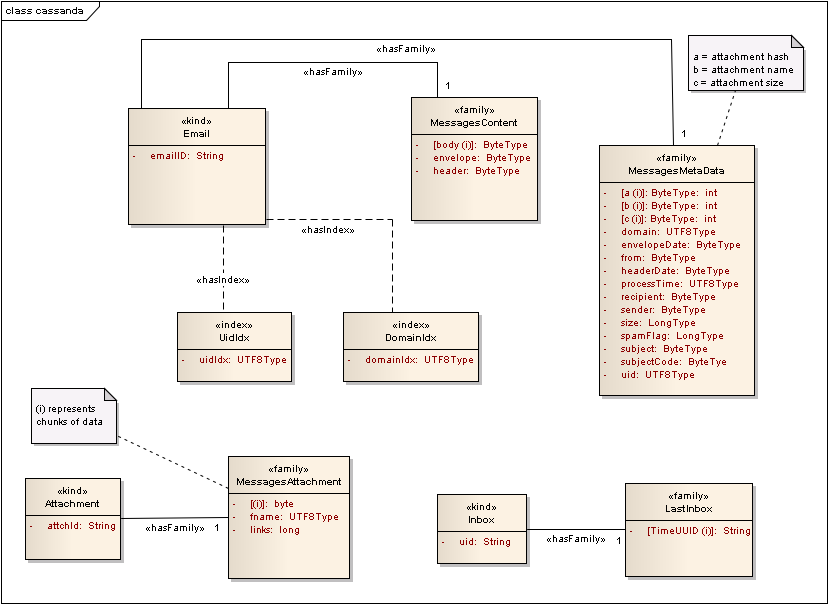
\includegraphics[width=17cm]{./figures/cassandra.png}
 % topologies802154.png: 722x407 pixel, 72dpi, 25.47x14.36 cm, bb=0 0 722 407
 \caption{Databázová schéma}
 \label{fig:Cschema}
\end{figure}

\section{Fultextové vyhľadávanie}

Fultextové vyhľadávanie realizujeme pomocou samostatného NoSQL systému Elasticsearch\footnote{http://elasticsearch.org}. Hlavný index, ktorý obsahuje všetky zaindexované dáta ma názov \emph{emailArchive}, a delíme ho na dva typy s názvom \emph{email} a \emph{envelope}. Schéma týchto typov obsahuje polia poďla, ktorých chceme v emailovom archíve vyhľadávať a jej reprezentáciu zapísanú vo formáte JSON znázorňuje obrázok \ref{fig:ESschema}.

\begin{figure}[h]
\begin{verbatim}
mappingsEmail = {
  "inbox": {"type": "string"},
  "from": {"type": "string"},
  "subject": {"type": "string"},
  "date" :{"type": "date"},
  "messageID" :{"type": "string", "index": "not_analyzed"},
  "attachments":{"type": "string"},
  "size": {"type": "long", "index": "not_analyzed"},
  "body": {"type": "string"}
}   
            
mappingsEnvelope = {
  "sender": {"type": "string"},
  "recipient": {"type": "string"},
  "ip": {"type": "ip"},
  "date": {"type": "date"}
}     
\end{verbatim}
 \caption{JSON schéma pre fultextové vyhľadávanie}
 \label{fig:ESschema}
\end{figure}      


\section{Implementácia}

%Consistent rad - write    W  + R > RF
V programovacom jazyku Python sme implementovali klienta pre zápis dát do databáze Cassandra a ElasticSearch. Jednou z najdoležitejších vlastností týchto klientov je voľba úrovne konzistencie pri zápise. Našou prioritou je integrita dát a od databáze požadujeme silnú konzistenciu. Zvolili sme mód kvóra (quorum), ktorý zabezpečí zápis dát na N / 2 + 1 replík a klient následne obdrží potvrdenie o úspešnosti zápisu, inak sa zápis zopakuje. Tieto vlastnosti nám zabezpečujú, v prípade použitia faktoru replikácie tri (dáta sa v databázovom systéme nachádzajú trikrát), silnú úroveň konzistencie na strane klienta a databáze. Analýza emailovej správy a jej deduplikácia spotrebúva hlavne CPU zdroje. Moderné procesory obsahuju viacero jadier, tento fakt môžeme využiť pre paralelizované spracúvanie emailov, teda každé jadro CPU bude spracúvať súčasne jednu emailovú správu.

\subsection*{Celery}
Paralelizáciu našej aplikácie sme zabezpečili pomocou využitia asynchrónnej fronty úloh pod názvom Celery\footnote{http://celeryproject.org}, ktorá využíva architektúru distribuovaného predávania správ (distributed message passing). Architektúru znázorňuje obrázok \ref{fig:Celery}. \uv{Pracovníci} (workers) reprezentujú samostatné procesy v našom prípade proces pre analýzu a deduplikáciu emailu, ktoré môžu bežať paralelne. Ako sprostredkovateľ (broker) je použitá aplikácia RabbitMQ\footnote{http://www.rabbitmq.com}. Sprostredkovateľ obdrží od klienta správu a uloží ju do fronty. Správa obsahuje identifikátor emailovej správy, v tomto prípade cestu na lokálnom súborovom systéme k súboru reprezentujúcom email. Táto správa je následne zaslaná ľubovoľnému pracovníkovy (v našom prípade klient vykonávajúci analýzu a deduplikáciu emailu), ktorý ju spracuje. Táto architektúra je plne distribuovaná, dokáže odolávať chybám (napr. v prípade výpadku elektrickej energie správy nadalej pretrvávajú vo fronte).

%TODO:
\begin{figure}[h]
 \centering
 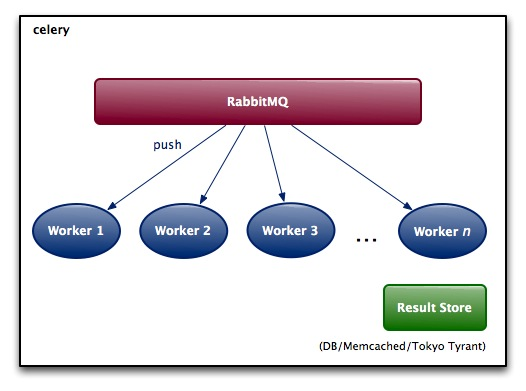
\includegraphics[width=10cm]{./figures/Celery.jpg}
 \caption{Architektúra Celery, Zdroj: [online], http://ask.github.com/celery/getting-started/introduction.html}
 \label{fig:Celery}
\end{figure}

Frontu RabbitMQ sme podrobili výkonnostnému testu, zvládala XY operácií pre zápis a XY pre načitanie správ.

\subsection{Klient}

Proces spracovania nového emailu je znázornený pomocou sekvenčného diagramu na obrázku \ref{fig:Cseq}. Pri príchode nového emailu, ktorý je spracovaný emailovým serverom Qmail, je vytvorená nová úloha pomocou aplikácie Celery. Táto úloha uloží do sprostredkovateľa identifikátor emailu. V prípade, že je v daný okamžik k dispozícií ľubovoľný pracovník, je emailová správa spracovaná pomocou nášho analyzátora a následne zapísaná do databáze Cassandra a fultextového systému Elasticsearch. Na testovacie účely sme nemali k dispozícii reálny dátový tok emailov. Vrstvu reprezentujúcu Qmail sme nahradili modulom, vytvárajúcim nové úlohy prechádzaním lokálneho súborového systému, ktorý obsahoval testovaciu množinu emailových správ.


\begin{figure}[h]
 \centering
 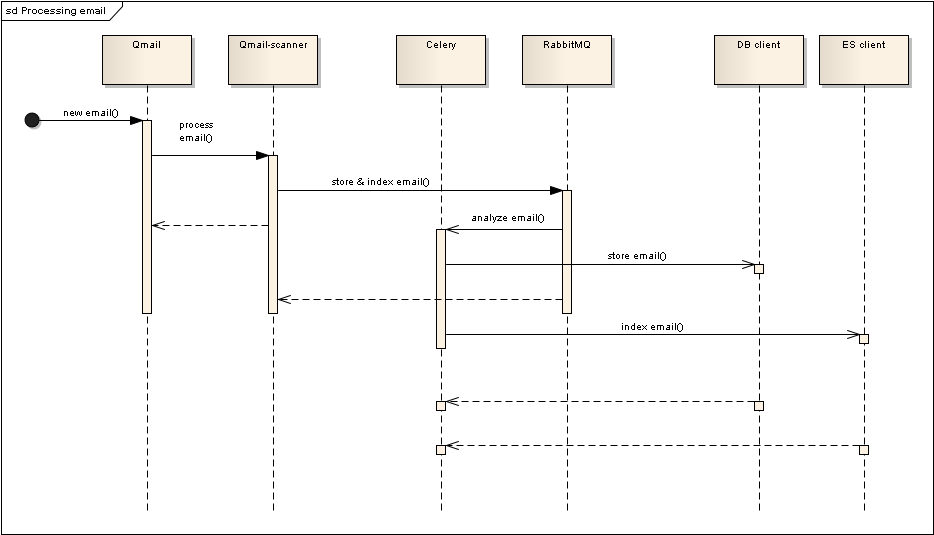
\includegraphics[width=16cm]{./figures/emailProcessing.png}
 % topologies802154.png: 722x407 pixel, 72dpi, 25.47x14.36 cm, bb=0 0 722 407
 \caption{Spracovanie emailu}
 \label{fig:Cseq}
\end{figure}


Návrh možnej realizácie daného riešenia je zachytený pomocou diagramu nasadenia na obrázku \ref{fig:Deployment}.
%deployment diagram ( oddelene datacentra - na tretej replikacii pocitat MR)ty?

\subsection{Výpočet štatistík}

%TODO PIG = kecy okolo 
% a nepodporuje možnosť definície viackrokového dátového toku \cite{Gates:2009:BHD:1687553.1687568}
Cassandra spolupracuje so systémom Hadoop, čo nám dáva do rúk mocný nástroj na masívne paralelné spracovanie dát pomocou techniky MapReduce. Tvorba aplikácií v tomto frameworku prebieha v Jave, je náročná a okrem toho programový model MapReduce obsahuje viaceo problémov. Model napríklad neobsahuje primitíva na filtrovanie, agregáciu, spájanie dát a je potrebná ich vlastná implementácia. Tieto nedostatky rieši nástroj Pig \cite{???} vďaka, ktorému sme boli schopný spracúvať metadáta uložené v databáze. Obrázok \ref{fig:PigExample} zobrazuje programovú ukážku, ktorá slúži na výpočet veľkosti najväčsieho emailu pre domény, ktorých emaily archivujeme. Pre jednoduchosť sme vynechali časti, ktoré slúžia na načítanie dát z databáze a obsahujú uživateľsky definovanú funkciu v programovacom jazyku Java, ktorá slúži na predprípravu vstupných dát. Podpora uživateľom definovaných funkcií je jednou z ďalších výhod nástroja Pig.

\begin{figure}[h]
\begin{verbatim}
notSpam = FILTER grp BY group.spam == 1;
maxSize = foreach grp {
  size = rows.size;
  generate group, MAX(size);
};
STORE maxSize into 'biggestEmailPerDomainDomain' using PigStorage(',');
\end{verbatim}
 \caption{Programová ukážka v jazyku Pig}
 \label{fig:PigExample}
\end{figure}  



\subsection{Webové rozhranie}
TODO
web IFACE -- pristup koncovych uzivatelov k archivu a diskusia ohladne bezpecnosti - strucny popis django aplikacie (topInbox, dumpInbox)



\section{Overenie návrhu}

Pomocou vyšie popísaného návrhu a implementovaných nástrojov sme overili funkčnosť nami navrhovaného modelu. Vhodná voľba daných verzií u aplikácií Celery a RabbiMQ bola určená počas písania a ladenia aplikácie. Všetky tieto aplikácie sú neustále vo vývoji, to isté platí pre databázu Cassandra a systém Hadoop. Počas písania tejto práce prebehlo viacero rozhovorov s autormi týchto aplikácii. Konkrétne databáza Cassandra na začiatku práce neobsahovala takmer žiadnu ucelenú dokumentáciu, počas začiatkov experimentov sme začínali s verziou 0.7.0. Počas ukončovania tejto práce je k dispozícii aktuálna verzia 0.7.5 a medzitým vznikla kvalitná online dokumentácia od spoločnosti Datastax\footnote{https://datastax.com}. 

\subsection*{Konfigurácia}
Hardverová konfigurácia bola totožná s konfiguráciou z kapitoly ???. Na šiestich serveroch bola nainštalovaná databáza Cassandra 0.7.3, Hadoop 0.20.2, dvojica serverov obsahovala klientskú aplikáciu a Celery 2.6. V úlohe sprostredkovateľa bola použitá aplikácia RabbitMQ 2.1.1, ktorá bola nainštalovaná na samostatnom serveri.


\subsection*{Overenie integrity dát}
Databázový kluster sme naplnili testovacími dátami obsahujúcimi emaily o objeme 300 GB. Následne sme simulovali prípad obnovy dát z archívu, kde sme všetky emaily v náhodnom poradí z databázy načítali, zostavili ich do pôvodného tvaru klientskou aplikáciou a porovnali sme ich odtlačok pomocou hašovacej funkcie MD5 s odtlačkom pôvodných dát uložených na pevnom disku. Tento test prebehol bez akejkoľvek chyby. 
Klient, ktorý slúžil na čítanie dát z databáze využíval mód kvóra, z dôvodu požiadavku na integritu dát.


\subsection*{Dosiahnuté výsledky}
Doležitým pozorovaním bol fakt, že z celkového objemu emailových správ 300 GB sa po deduplikácií príloh tento objem znížil na 99 GB, teda došlo k 67\% úspore diskovej kapacity. Štruktúry do ktorých sme ukladali dáta pre potrebu štatistík zaberali 0,4\% z celkového objemu dát, čo je zanedbateľná položka.

\noindent
ElasticSearch rychlost pre fultextové vyhladavanie bola do XY ms, indexy nad objemom dát 300 GB tvorili XY GB.

\section{Doporúčenie najvhodnejšieho systému}
Pouzit Brisk - nastupca Cassandry s nativnou podporou Hadoop-u, alebo nejaky key-value (to by bolo ale treba zanalyzovať a zmerat performance, je nutne to teda vobec spominat?)


%Rabbit rychlost

\chapter{Záver}


%kolko deduplikacia
%kolko MB attacch
%mapreduce - PIG
%popis vysledkov
%kolko tvorili indexy




%*****************************************************************************
% Seznam literatury je v samostatnem souboru reference.bib. Ten
% upravte dle vlastnich potreb, potom zpracujte (a do textu
% zapracujte) pomoci prikazu bibtex a nasledne pdflatex (nebo
% latex). Druhy z nich alespon 2x, aby se poresily odkazy.

\bibliographystyle{abbrv}
%bibliographystyle{plain}
%\bibliographystyle{psc}
{
%JZ: 11.12.2008 Kdo chce mit v techto ukazkovych odkazech take odkaz na CSTeX:
\def\CS{$\cal C\kern-0.1667em\lower.5ex\hbox{$\cal S$}\kern-0.075em $}
\bibliography{reference}
}

% M. Dušek radi:
%\bibliographystyle{alpha}
% kdy citace ma tvar [AutorRok] (napriklad [Cook97]). Sice to asi neni  podle ceske normy (BTW BibTeX stejne neodpovida ceske norme), ale je to nejprehlednejsi.
% 3.5.2009 JZ polemizuje: BibTeX neobvinujte, napiste a poskytnete nam styl (.bst) splnujici citacni normu CSN/ISO.

%*****************************************************************************
%*****************************************************************************
\appendix


%*****************************************************************************

\chapter{Zoznam použitých skratiek}
\begin{description}

\item[API] - 
\item[JVM]
\item[NoSQL]
\item[PB]
\item[RFC]
\item[SPOF]
\end{description}
\vdots

%*****************************************************************************
\chapter{UML diagramy}


\begin{figure}[h]
 \centering
 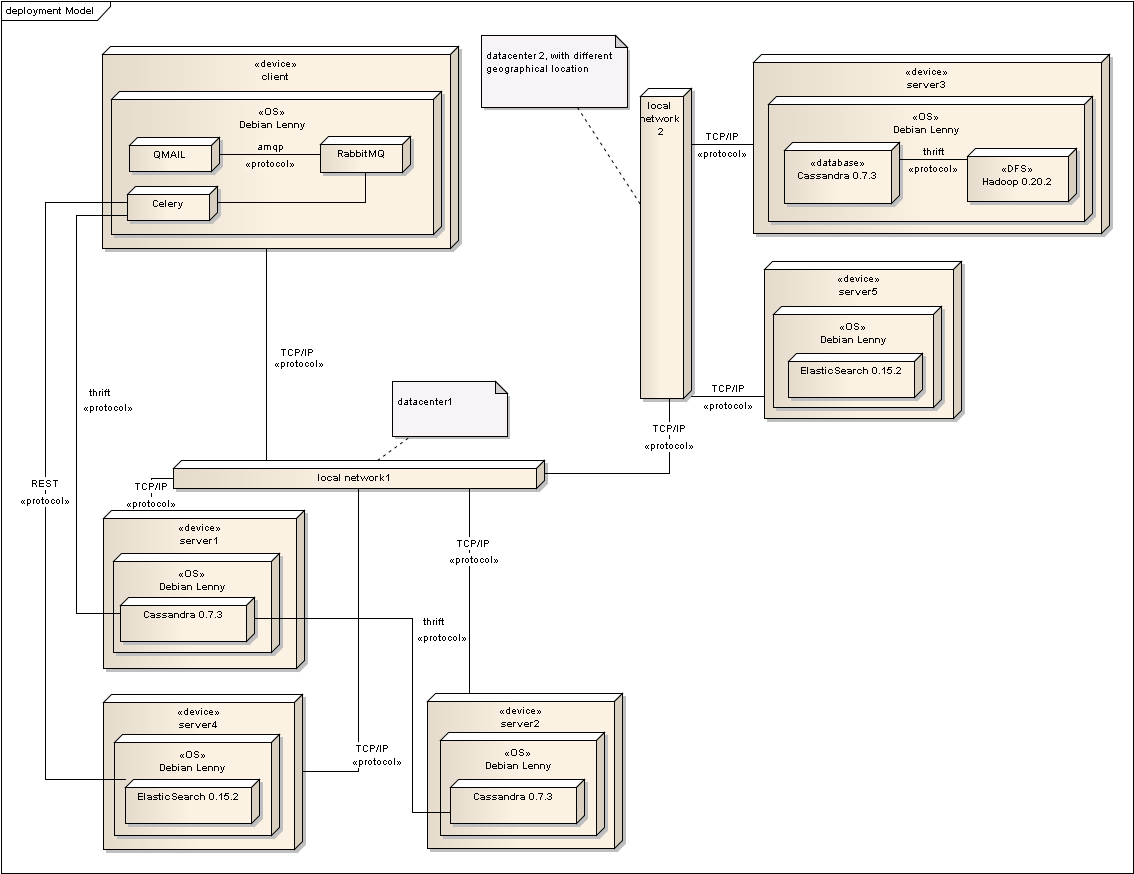
\includegraphics[width=16cm]{./figures/deploy.png}
 \caption{Diagram nasadenia aplikácie}
 \label{fig:Deployment}
\end{figure}

%*****************************************************************************

\chapter{Inštalačná a užívateľská príručka}
\textbf{\large Tato příloha velmi žádoucí zejména u softwarových implementačních prací.}

%*****************************************************************************

\chapter{Obsah priloženého CD}
\textbf{\large Tato příloha je povinná pro každou práci. Každá práce musí totiž obsahovat přiložené CD. Viz dále.}

Může vypadat například takto. Váš seznam samozřejmě bude odpovídat typu vaší práce. (viz \cite{infodp}):

\begin{figure}[h]
\begin{center}
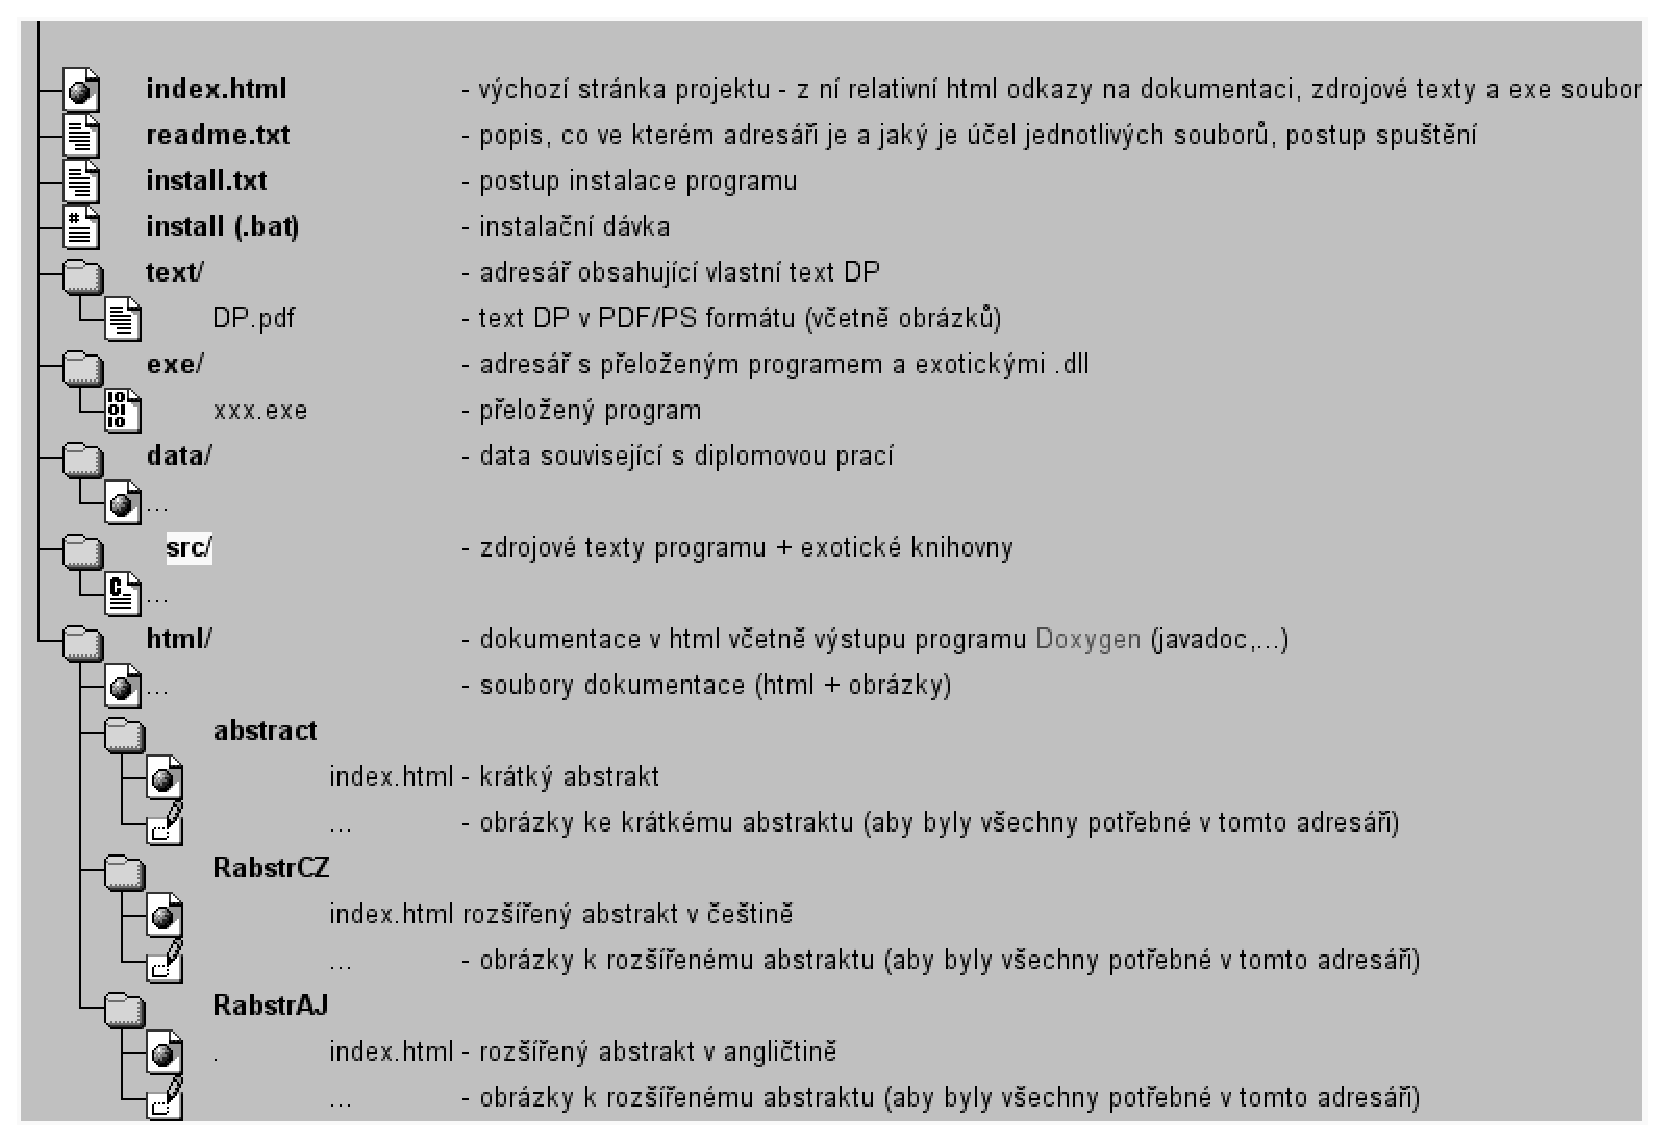
\includegraphics[width=14cm]{figures/seznamcd}
\caption{Seznam přiloženého CD --- příklad}
\label{fig:seznamcd}
\end{center}
\end{figure}

Na GNU/Linuxu si strukturu přiloženého CD můžete snadno vyrobit příkazem:\\ 
\verb|$ tree . >tree.txt|\\
Ve vzniklém souboru pak stačí pouze doplnit komentáře.

Z \textbf{README.TXT} (případne index.html apod.)  musí být rovněž zřejmé, jak programy instalovat, spouštět a jaké požadavky mají tyto programy na hardware.

Adresář \textbf{text}  musí obsahovat soubor s vlastním textem práce v PDF nebo PS formátu, který bude později použit pro prezentaci diplomové práce na WWW.

\end{document}
